% Options for packages loaded elsewhere
% Options for packages loaded elsewhere
\PassOptionsToPackage{unicode}{hyperref}
\PassOptionsToPackage{hyphens}{url}
\PassOptionsToPackage{dvipsnames,svgnames,x11names}{xcolor}
%
\documentclass[
]{article}
\usepackage{xcolor}
\usepackage{amsmath,amssymb}
\setcounter{secnumdepth}{-\maxdimen} % remove section numbering
\usepackage{iftex}
\ifPDFTeX
  \usepackage[T1]{fontenc}
  \usepackage[utf8]{inputenc}
  \usepackage{textcomp} % provide euro and other symbols
\else % if luatex or xetex
  \usepackage{unicode-math} % this also loads fontspec
  \defaultfontfeatures{Scale=MatchLowercase}
  \defaultfontfeatures[\rmfamily]{Ligatures=TeX,Scale=1}
\fi
\usepackage{lmodern}
\ifPDFTeX\else
  % xetex/luatex font selection
  \setmainfont[]{Verdana}
\fi
% Use upquote if available, for straight quotes in verbatim environments
\IfFileExists{upquote.sty}{\usepackage{upquote}}{}
\IfFileExists{microtype.sty}{% use microtype if available
  \usepackage[]{microtype}
  \UseMicrotypeSet[protrusion]{basicmath} % disable protrusion for tt fonts
}{}
\makeatletter
\@ifundefined{KOMAClassName}{% if non-KOMA class
  \IfFileExists{parskip.sty}{%
    \usepackage{parskip}
  }{% else
    \setlength{\parindent}{0pt}
    \setlength{\parskip}{6pt plus 2pt minus 1pt}}
}{% if KOMA class
  \KOMAoptions{parskip=half}}
\makeatother
% Make \paragraph and \subparagraph free-standing
\makeatletter
\ifx\paragraph\undefined\else
  \let\oldparagraph\paragraph
  \renewcommand{\paragraph}{
    \@ifstar
      \xxxParagraphStar
      \xxxParagraphNoStar
  }
  \newcommand{\xxxParagraphStar}[1]{\oldparagraph*{#1}\mbox{}}
  \newcommand{\xxxParagraphNoStar}[1]{\oldparagraph{#1}\mbox{}}
\fi
\ifx\subparagraph\undefined\else
  \let\oldsubparagraph\subparagraph
  \renewcommand{\subparagraph}{
    \@ifstar
      \xxxSubParagraphStar
      \xxxSubParagraphNoStar
  }
  \newcommand{\xxxSubParagraphStar}[1]{\oldsubparagraph*{#1}\mbox{}}
  \newcommand{\xxxSubParagraphNoStar}[1]{\oldsubparagraph{#1}\mbox{}}
\fi
\makeatother


\usepackage{longtable,booktabs,array}
\newcounter{none} % for unnumbered tables
\usepackage{calc} % for calculating minipage widths
% Correct order of tables after \paragraph or \subparagraph
\usepackage{etoolbox}
\makeatletter
\patchcmd\longtable{\par}{\if@noskipsec\mbox{}\fi\par}{}{}
\makeatother
% Allow footnotes in longtable head/foot
\IfFileExists{footnotehyper.sty}{\usepackage{footnotehyper}}{\usepackage{footnote}}
\makesavenoteenv{longtable}
\usepackage{graphicx}
\makeatletter
\newsavebox\pandoc@box
\newcommand*\pandocbounded[1]{% scales image to fit in text height/width
  \sbox\pandoc@box{#1}%
  \Gscale@div\@tempa{\textheight}{\dimexpr\ht\pandoc@box+\dp\pandoc@box\relax}%
  \Gscale@div\@tempb{\linewidth}{\wd\pandoc@box}%
  \ifdim\@tempb\p@<\@tempa\p@\let\@tempa\@tempb\fi% select the smaller of both
  \ifdim\@tempa\p@<\p@\scalebox{\@tempa}{\usebox\pandoc@box}%
  \else\usebox{\pandoc@box}%
  \fi%
}
% Set default figure placement to htbp
\def\fps@figure{htbp}
\makeatother


% definitions for citeproc citations
\NewDocumentCommand\citeproctext{}{}
\NewDocumentCommand\citeproc{mm}{%
  \begingroup\def\citeproctext{#2}\cite{#1}\endgroup}
\makeatletter
 % allow citations to break across lines
 \let\@cite@ofmt\@firstofone
 % avoid brackets around text for \cite:
 \def\@biblabel#1{}
 \def\@cite#1#2{{#1\if@tempswa , #2\fi}}
\makeatother
\newlength{\cslhangindent}
\setlength{\cslhangindent}{1.5em}
\newlength{\csllabelwidth}
\setlength{\csllabelwidth}{3em}
\newenvironment{CSLReferences}[2] % #1 hanging-indent, #2 entry-spacing
 {\begin{list}{}{%
  \setlength{\itemindent}{0pt}
  \setlength{\leftmargin}{0pt}
  \setlength{\parsep}{0pt}
  % turn on hanging indent if param 1 is 1
  \ifodd #1
   \setlength{\leftmargin}{\cslhangindent}
   \setlength{\itemindent}{-1\cslhangindent}
  \fi
  % set entry spacing
  \setlength{\itemsep}{#2\baselineskip}}}
 {\end{list}}
\usepackage{calc}
\newcommand{\CSLBlock}[1]{\hfill\break\parbox[t]{\linewidth}{\strut\ignorespaces#1\strut}}
\newcommand{\CSLLeftMargin}[1]{\parbox[t]{\csllabelwidth}{\strut#1\strut}}
\newcommand{\CSLRightInline}[1]{\parbox[t]{\linewidth - \csllabelwidth}{\strut#1\strut}}
\newcommand{\CSLIndent}[1]{\hspace{\cslhangindent}#1}



\setlength{\emergencystretch}{3em} % prevent overfull lines

\providecommand{\tightlist}{%
  \setlength{\itemsep}{0pt}\setlength{\parskip}{0pt}}



 


\usepackage{orcidlink,fancyhdr,graphicx,xcolor,xstring,fontspec,mdframed}
\usepackage[margin=1in]{geometry}
\usepackage[onehalfspacing]{setspace}
\usepackage[scale=2.5]{ccicons}
\definecolor{SRXIVgreen}{RGB}{207, 250, 209}
\newcommand\shortauthor{}
\usepackage{fontspec}
\usepackage{multirow}
\usepackage{multicol}
\usepackage{colortbl}
\usepackage{hhline}
\newlength\Oldarrayrulewidth
\newlength\Oldtabcolsep
\usepackage{longtable}
\usepackage{array}
\usepackage{hyperref}
\usepackage{float}
\usepackage{wrapfig}
\makeatletter
\@ifpackageloaded{caption}{}{\usepackage{caption}}
\AtBeginDocument{%
\ifdefined\contentsname
  \renewcommand*\contentsname{Table of contents}
\else
  \newcommand\contentsname{Table of contents}
\fi
\ifdefined\listfigurename
  \renewcommand*\listfigurename{List of Figures}
\else
  \newcommand\listfigurename{List of Figures}
\fi
\ifdefined\listtablename
  \renewcommand*\listtablename{List of Tables}
\else
  \newcommand\listtablename{List of Tables}
\fi
\ifdefined\figurename
  \renewcommand*\figurename{Figure}
\else
  \newcommand\figurename{Figure}
\fi
\ifdefined\tablename
  \renewcommand*\tablename{Table}
\else
  \newcommand\tablename{Table}
\fi
}
\@ifpackageloaded{float}{}{\usepackage{float}}
\floatstyle{ruled}
\@ifundefined{c@chapter}{\newfloat{codelisting}{h}{lop}}{\newfloat{codelisting}{h}{lop}[chapter]}
\floatname{codelisting}{Listing}
\newcommand*\listoflistings{\listof{codelisting}{List of Listings}}
\makeatother
\makeatletter
\makeatother
\makeatletter
\@ifpackageloaded{caption}{}{\usepackage{caption}}
\@ifpackageloaded{subcaption}{}{\usepackage{subcaption}}
\makeatother
\usepackage{bookmark}
\IfFileExists{xurl.sty}{\usepackage{xurl}}{} % add URL line breaks if available
\urlstyle{same}
\hypersetup{
  pdfauthor={Gorman, B.T.; Impellizzeri, F.M.; Warne, J.},
  pdfkeywords={hypothesis testing, falsifiability, severity, sport and
exercise science},
  colorlinks=true,
  linkcolor={blue},
  filecolor={Maroon},
  citecolor={Blue},
  urlcolor={blue},
  pdfcreator={LaTeX via pandoc}}


\author{Gorman, B.T. \and Impellizzeri, F.M. \and Warne, J.}
\date{}
\begin{document}

% set short author name
\newcounter{nauthor}
\stepcounter{nauthor}\stepcounter{nauthor}\stepcounter{nauthor}
\ifnum\thenauthor>2
\renewcommand{\shortauthor}{Gorman, B.T. et al. }
\else 
\renewcommand{\shortauthor}{Gorman \& Impellizzeri \& Warne }
\fi

\pagestyle{fancy}
\fancyhead[L]{\shortauthor(\the\year)}
\fancyhead[R]{}
\fancypagestyle{firstpage}{
  \fancyhf{}% clear default for head and foot
  \lhead{\href{https://sportrxiv.org}{
\includegraphics[width = 40mm]{logo.png}}}
  \chead{PREPRINT - NOT PEER REVIEWED}
  \rhead{\ccby\vspace{0.2mm}}
  \lfoot{\color{gray}All authors have read and approved  this version  of the manuscript. \linebreak The manuscript was last updated on \today}
}
\begin{flushleft}
\begin{spacing}{2.5}
\thispagestyle{firstpage}
\vspace*{0.1cm}
{\huge{\textbf{Hypotheses in Name Only? An Examination of Hypothesis
Statements in Sport and Exercise Science Research}}}
\end{spacing}
\vspace*{0.1cm}
Gorman,
B.T.\textsuperscript{1*}~\orcidlink{0009-0006-4318-5430}, Impellizzeri,
F.M.\textsuperscript{2}~\orcidlink{0000-0002-1703-2573}, Warne,
J.\textsuperscript{1}~\orcidlink{0000-0002-4359-8132}
\\
\bigskip
\textsuperscript{1}School of Biological, Health and Sport Sciences,
Technological University Dublin, Tallaght Campus, Dublin,
Ireland.\\ \textsuperscript{2}Human Performance Research Centre, School
of Sport, Exercise and Rehabilitation, University of Technology Sydney,
Ultimo, Australia.
\\
\bigskip
*Correspondence: 
\href{mailto:barrytgorman@gmail.com}{\color{black}barrytgorman@gmail.com}
\\
\bigskip
\begin{spacing}{1}
Cite as: \shortauthor(\the\year). Hypotheses in Name Only? An
Examination of Hypothesis Statements in Sport and Exercise Science
Research. \emph{SportRxiv.} \\
\end{spacing}
  \vspace{1mm} Supplementary Materials: \href{https://osf.io/}{https://osf.io/} \\
\vspace*{1cm}
\end{flushleft}


\newenvironment{abstractbox}
  {}

\surroundwithmdframed[
  backgroundcolor=SRXIVgreen,
  innertopmargin=10pt,
  innerbottommargin=10pt,
  linewidth=2pt,
  linecolor=gray!30,
  leftmargin=20pt,
  rightmargin=20pt,
  frametitle={\large{Abstract}},
]{abstractbox}

\begin{abstractbox}
  The replication rate in sport and exercise science was recently
estimated to be twenty-eight percent, and the majority of the field's
metascientific work has focused on statistical and methodological
issues. We argue that these concerns are secondary to a prior concern:
whether the hypotheses being tested are falsifiable and informative to
begin with. Hypotheses in sport and exercise science appear to be
underspecified. So underspecified in fact that almost any outcome can be
reconciled with them. These hypotheses may replicate readily but tell us
very little, because a test carries evidential weight only to the extent
the hypothesis could have failed it. Therefore, as a supplement to a
larger project (see preregistration Gorman et al.~(2024)), we conducted
a qualitative content analysis, using NVivo (version 14), of hypothesis
statements from 269 research articles published in quartile one sport
and exercise science journals. We primarily examine four features of the
hypothesis statements that bear on the severity of the test: their
structure, their dependent variables and summary measures, and their
directionality. We also discuss the claims researchers make after
testing their hypotheses. 
    \\ \\
  Keywords: \emph{hypothesis testing; falsifiability; severity; sport
and exercise science}
   
\end{abstractbox}

\section{Introduction}\label{introduction}

The estimated replication rate in sport and exercise science is
twenty-eight percent (95\% CI {[}12.9\%, 49.6\%{]})
(\citeproc{ref-murphy_estimating_2025}{Murphy et al., 2025}). That is,
twenty-eight percent of replications returned a statistically
significant effect in the same direction and of similar magnitude to the
original. This is a legitimate concern, but we will argue that the
replication rate is not the field's most fundamental problem, because it
is largely insensitive to the quality of the hypotheses being tested. To
understand why, consider the \emph{inverse}. Would a higher replication
rate of 70\%, for example, reassure us? Our answer is: it depends. More
specifically, it depends on the hypothesis being tested (amongst other
dependencies). Replication \emph{success} is defined by statistical
criteria (typically significance and effect-size consistency); it
indicates that a result may be reliably replicable, but it typically
provides limited information about the quality or informativeness of the
underlying hypothesis itself.

A hypothesis with a low degree of falsifiability i.e.~so weakly
specified that almost any outcome can be reconciled with it, could yield
results that replicate readily while telling us little. Weak predictions
of this kind are both easy to confirm and, if real, straightforward to
reproduce; as such, a high replication rate obtained this way would not
place the field in a better position in the development of knowledge. A
test carries evidential weight only to the extent that the hypothesis
could have failed it (\citeproc{ref-mayo_statistical_2018}{Mayo, 2018});
replicating a non-severe test merely reproduces a non-severe test. In
our view, replications are important, but there is little value in
replicating a study whose hypothesis is so underspecified that the
result, whatever it turns out to be, is uninformative.

This is why we view the hypothesis problem as logically prior to the
methodological one. The meta-scientific literature appears to have
primarily focused on the various methodological and statistical issues
of the field (for example: lack of statistical power
(\citeproc{ref-mesquida_replication_2022}{Mesquida et al., 2022};
\citeproc{ref-mesquida_replicability_2025}{Mesquida, Murphy, et al.,
2025}), small sample sizes (\citeproc{ref-abt_power_2020}{Abt et al.,
2020}, \citeproc{ref-abt_sample_2025}{2025};
\citeproc{ref-mccrum_sample_2022}{McCrum et al., 2022};
\citeproc{ref-mckay_low_2022}{McKay et al., 2022};
\citeproc{ref-mesquida_publication_2023}{Mesquida et al., 2023};
\citeproc{ref-twomey_nature_2021}{Twomey et al., 2021})). However,
little specific attention (with the exception of Mesquida, Warne, et al.
(\citeproc{ref-mesquida_what_2025}{2025})) has been given to the
hypotheses being tested in sport and exercise science research. Concerns
about sample size and statistical power are secondary to concerns about
whether the hypotheses being tested are falsifiable and informative to
begin with. A necessary first step, then, is to examine the hypotheses
we are actually testing in the literature.

This paper is part of a larger project (see preregistration Gorman et
al. (\citeproc{ref-gorman2024}{2024})), and the `hypotheses' we discuss
here were extracted from 269 articles within quartile one sport and
exercise science journals. More specifically, our field rarely
explicitly states statistical hypotheses and therefore, we only assumed
them as hypotheses when researchers made it explicit that they had
`expectations' from the data. That is, they stated ``\emph{we
hypothesized\ldots{}}'', ``\emph{it was hypothesized\ldots{}}''
``\emph{we expected\ldots{}}'', ``\emph{we predicted\ldots{}}'', for
example, at the end of the introduction section. This excludes
expectations that are implied but never stated. The exclusion is
conservative, but the hypothesis statements we have analysed are those
the authors themselves marked as hypotheses. The problems we identify
are therefore problems with the field's most explicit theoretical
commitments, not commitments we have attributed to the authors. Further,
the issues discussed here can also be relevant to other statistical
approaches (e.g.~Bayesian) as long as substantive hypotheses are
explicitly stated.

Intentionally or not, sport and exercise research appears to have
largely `landed' on hypothesis testing as \emph{the} method of
statistical inference (\citeproc{ref-buttner_are_2020}{Büttner et al.,
2020}; \citeproc{ref-twomey_nature_2021}{Twomey et al., 2021}).
Specifically, it appears that the majority of researchers are adopting
the Neyman-Pearson approach to null-hypothesis significance testing
(NHST). This approach is intended to support reliable, scientific claims
whilst controlling long-run error rates
(\citeproc{ref-neyman1928}{Neyman \& Pearson, 1928}). The approach first
requires a hypothesis \emph{H} and relies on a premise that tests of
\emph{H} should be capable of revealing that \emph{H} is false if it is
in fact false. That is, the tests should be appropriately stringent or
`severe' and follow the severity requirement
(\citeproc{ref-mayo_statistical_2018}{Mayo, 2018}), where: ``\emph{One
does not have evidence for a claim if nothing has been done to rule out
ways the claim may be false.}''
(\citeproc{ref-mayo_statistical_2018}{Mayo, 2018, p. 5}). When our
\emph{H} has survived a severe test, the verisimilitude (or
`truth-likeness') of our theory\footnote{A theory is not a guess or
  hunch. It is a ``\emph{vehicle of scientists' understanding of
  phenomena}'' (\citeproc{ref-van_lissa_be_2026}{Van Lissa et al., 2026,
  p. 4}).

  Further, for clarity, Mayo's `error-statistical' account warrants
  ``this claim has passed a stringent test'' not ``the theory is closer
  to the truth''.} is considerably increased or decreased. This
severity, however, is reliant on ``\emph{all characteristics of a
study}'' (\citeproc{ref-lakens2019}{Lakens, 2019, p. 224}), but in this
article we will discuss severity relative to the: hypothesis structure,
hypothesis dependent variables and summary measures, and hypothesis
directionality. We will also discuss the claims researchers make
regarding their hypotheses. It is important to point out that we
primarily relate these issues to their impact on statistical
significance, not practical significance which is another very important
aspect however not covered in the current article (see Mesquida, Warne,
et al. (\citeproc{ref-mesquida_what_2025}{2025}) for more on this). User
friendly, practical examples will be provided, with some necessary
simplifications, with the aims of making researchers aware of these
issues and educating them on ways to improve the consistency and logic
in their approach to hypothesis formulation and testing. As mentioned,
this paper is a supplement to a larger project (see preregistration
Gorman et al. (\citeproc{ref-gorman2024}{2024})) and to aid this current
article we specifically conducted post-hoc qualitative analysis (using
NVivo, version 14) on each of the 269 studies published in quartile one
journals between January 2019 and May 2024. We will try to cover
multiple observed concerns, some of which would require further
elaboration beyond the scope of this article. Therefore, it should be
considered, in a sense, a summary of sorts.

\section{First, do we ask risky
questions?}\label{first-do-we-ask-risky-questions}

``\emph{One can inquire as to why this is, whether anything can be done
about it, or -- a question that should be asked first -- does it really
matter anyway?}'' (\citeproc{ref-meehl_psychology_1986}{Meehl, 1986, p.
4})

To begin, in some cases it appears that sport and exercise science
researchers could be accused of having hypotheses which examine `low
hanging fruit', i.e.~hypotheses being framed such that corroboration is
the most likely outcome. That is, a hypothesis may be severe and stated
precisely but ultimately not risky. We have coined this tendency
`CASHing' (Corroboration-Assured Selection of Hypotheses): researchers
cashing by (conveniently) selecting hypotheses with such high \emph{a
priori} plausibility, that corroboration is near-assured, and the test
is unlikely to fail. Unlike HARKing (Hypothesizing After the Results are
Known) (\citeproc{ref-kerr1998}{Kerr, 1998}), where the hypothesis is
formulated after the results are known, CASHing operates in advance: the
hypothesis is genuine and pre-specified, but chosen precisely because it
is almost certain to be confirmed. From a probabilistic perspective,
this is the most effective way of increasing the chance of
corroboration. For example, if we conduct 100 separate studies with the
typical alpha (5\%) and power (80\%) levels and our H\textsubscript{0}
has a 70\% probability of being true, then in the long run, 24\% of the
100 studies will be true positives. Whereas if we do not change the
alpha and power but decrease the probability of H\textsubscript{0} being
true to 10\% - increasing the probability of H\textsubscript{1} being
true from 30\% to 90\% - then, in the long run, 72\% of the 100 studies
will be true positives.

With this in mind, and inspired by the weather prediction example of
Meehl (\citeproc{ref-meehl_appraising_1990}{1990}) {[}p.~110{]} and
figure 5.3 of Lakens (\citeproc{ref-lakens_improving_2022}{2022, pp.
116--117}), we have created a practical example of CASHing specific to
sport and exercise science. We have two sport scientists, let's call
them Sport Scientist A and Sport Scientist B, who are supervising one of
their athletes (Athlete 1) performing a single counter-movement jump.
Athlete 1 is very `athletic', but this is his first time completing a
counter-movement jump on force plates. Before Athlete 1 performs the
jump, both sport scientists verbalise a `hypothesis' to each other:

\begin{center}

Sport Scientist A: "\textit{Athlete 1 will have a jump height greater than 0cm}"

Sport Scientist B: "\textit{Athlete 1 will have a jump height greater than or equal to 40.0cm and less than or equal to 42.0cm}"

\end{center}

Without asking the scientists to formalize their statistical hypotheses
or knowing how high the athlete jumped, who has the riskier hypothesis?
(Examining \textbf{Figure 1} may help you answer this). It should be
obvious, it is Sport Scientist B. This is because the only means by
which the hypothesis of Sport Scientist A is not supported is if the
athlete cannot jump (slim red line on the left panel in \textbf{Figure
1}). This is extremely unlikely given that Athlete 1 is (obviously) an
athlete and therefore should be able to jump. Ultimately, the hypothesis
of Sport Scientist A has a very high probability of being corroborated,
and Sport Scientist A can be considered to be CASHing. This may appear
as an exaggerated example but from our coding of the sport and exercise
science literature, we have seen multiple examples not far from this.
Here is one such example taken from the literature:

\begin{center}

"\textit{It is hypothesised that positional differences will exist for technical and running performance and that there will be a distinct difference between competition grades for technical and running performance}."

\end{center}

In the case of the above hypothesis, it is not risky, it only predicts
that \emph{differences} will exist between positions and competition
grades, despite there already being strong grounds to expect such
differences based on positional demands and level of play.

Therefore, it is important for researchers to bear in mind that in some
cases, a hypothesis test may not be useful to answer your given
question. Lakens (\citeproc{ref-lakens_improving_2022}{2022, p. 120})
proposes that a hypothesis test is `useful' when: 1) ``\emph{both data
generating models that are decided between} {[}are mutually exclusive
and{]} \emph{have some plausibility}'' and 2) ``\emph{it is possible to
employ an informative} {[}objective{]} \emph{methodological procedure}''
(bracketed inserts are ours). Taking this into account, Sport Scientist
A's hypothesis falls at point 1. It is not a particularly informative
hypothesis (Athlete 1 jumped 41.3cm). In comparison, if we do believe
testing a hypothesis is warranted then we must follow - because we
should also subscribe to following point 2 - Sport Scientist B and make
a risky prediction: a prediction where we emerge astounded if something
emerges from the noise. In summary, if a hypothesis is not risky, it
places little constraint on what counts as supporting or dis-confirming
evidence. As a result, it is less falsifiable, less informative, and
less capable of advancing theory. To clarify, there are settings where a
more generic hypothesis is appropriate, for example, in genuinely
exploratory work, where the aim is to generate hypotheses rather than
test them. What matters is that such work is labelled as exploratory and
not presented as a confirmatory test. Any exploratory hypothesis
testing, is therefore better understood as a descriptive flag to
identify what might be worth subjecting to more severe testing later.
The concern we raise here applies to `confirmatory' research, where the
hypothesis should be specific, determined \emph{a-priori}, and
falsifiable.

\begin{figure}[H]

{\centering \pandocbounded{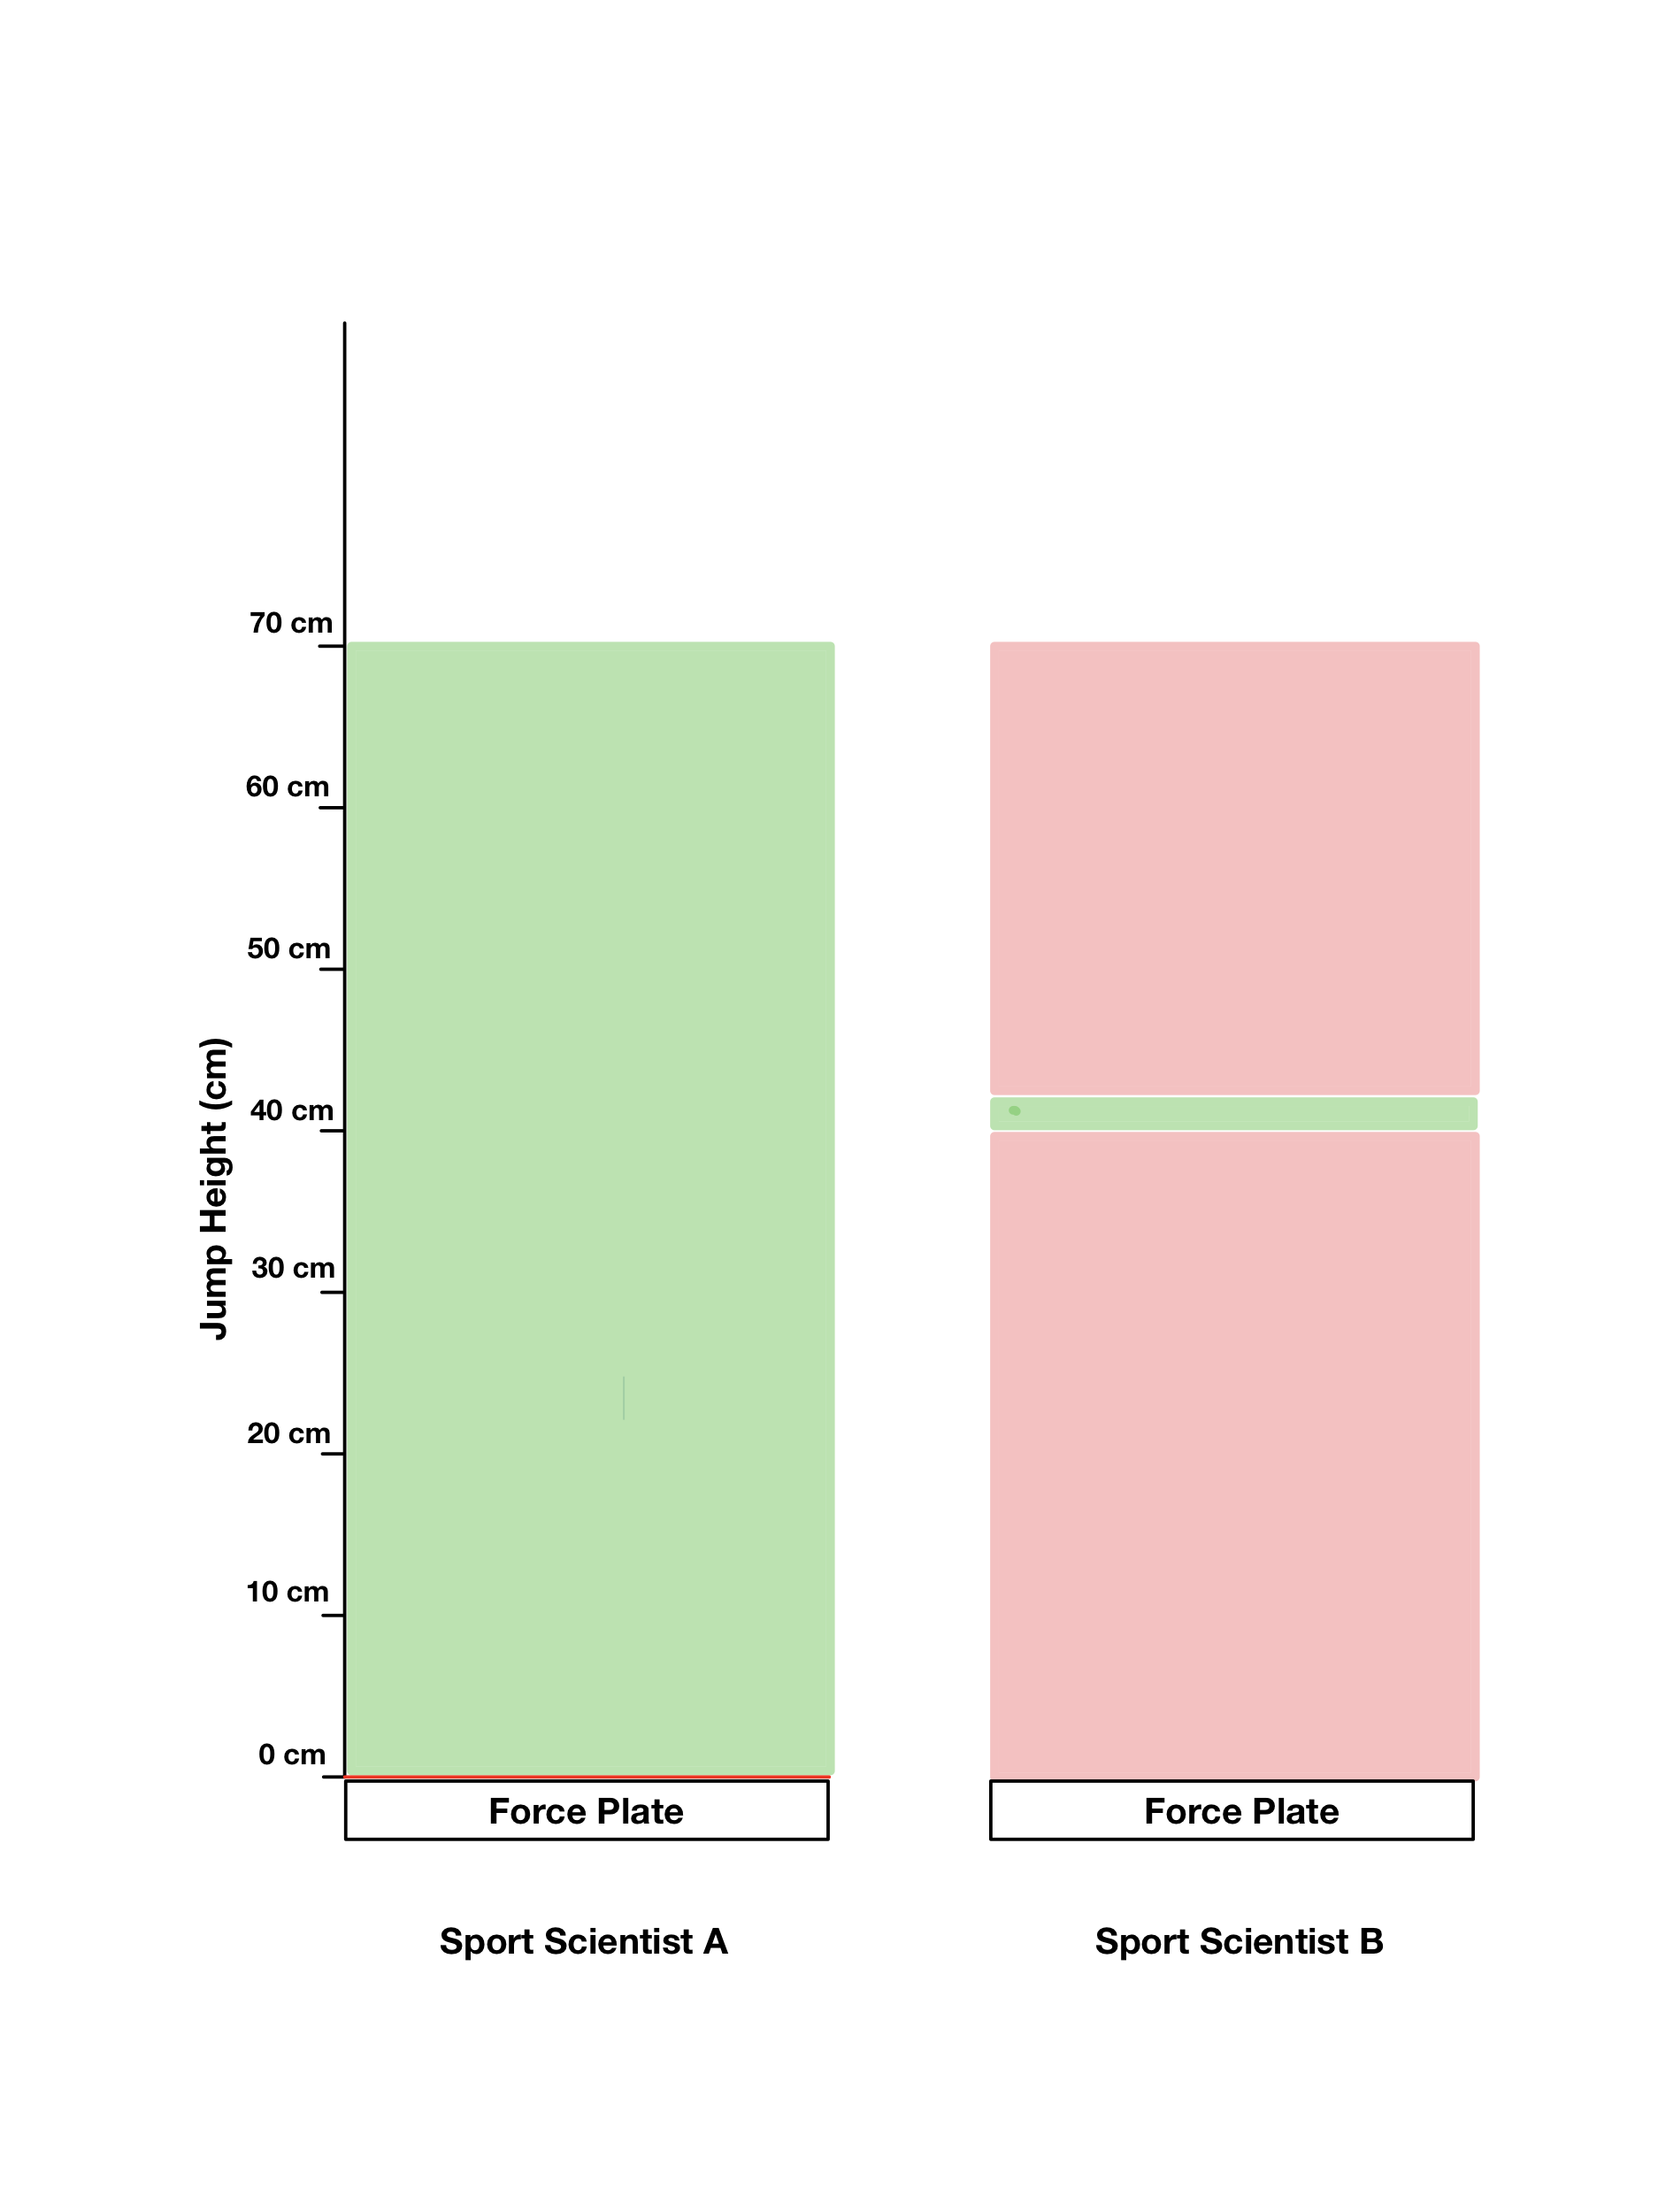
\includegraphics[keepaspectratio]{figures/figure_1.png}}

}

\caption{The hypothesis of Sport Scientist A and the hypothesis Sport
Scientist B. Green zone: area of claimed `support' for hypotheses. Red
line and red zone: area(s) of claimed `no support' for hypotheses. Image
created by BG using Notability (Ginger Labs, Inc.~Version 16.7).}

\end{figure}%

The above examples, and all following examples, propose that hypotheses
are framed prior to data collection, but given the level of positive
results in our literature (\citeproc{ref-buttner_are_2020}{Büttner et
al., 2020}; \citeproc{ref-twomey_nature_2021}{Twomey et al., 2021}), it
would be naive to believe that a high proportion of hypotheses aren't
simply produced by HARKing. This can occur as \emph{a priori} hypotheses
being suppressed or altered if false, or ad-hoc hypotheses being
constructed after some exploration of the data. While HARKed hypotheses
may still be true, they are not severe tests as they have been derived
from the data and thus can never be proven false. For the remainder of
this article, we will, perhaps naively, take the assumption that the
observed hypotheses have not been HARKed. Firstly, we do this because
this practice is almost impossible to detect in the absence of
preregistration and transparency, and secondly because we need to
promote concepts of principled hypothesis construction, theoretically
constrained operationalisation, and meaningful falsifiability,
independent of researchers analytic flexibility. Lastly, we want to
highlight that just because a hypothesis was created prior to looking at
the data does not equate it to a severe test, as we will see. To begin,
we present a conversation on the very structure of hypothesis statements
in sport and exercise science research.

\section{The Structure of Hypothesis
Statements}\label{the-structure-of-hypothesis-statements}

Firstly, if NHST is being utilized, then a researcher's \emph{H} should
first be separated into its statistical components, or formal `model':
H\textsubscript{1} (the affirmation of \emph{H}) and H\textsubscript{0}
(the refutation of \emph{H}). Sport and exercise science researchers
typically just state their \emph{H} using a `verbal' conjecture located
near the end of the introduction section:

\begin{center}

"\textit{It was hypothesized that acute caffeine supplementation would improve sprint performance}...".

\end{center}

More specifically, researchers typically employed the terminology
displayed in \textbf{Table 1}. These verbal statements are a logical
starting point for anything we wish to study. However, when we state our
hypotheses, we must attempt to narrow the scope of what we exactly mean.
If researchers just state \emph{H} as a verbal conjecture with no
explicit reference to H\textsubscript{1}, then it is difficult to find
evidence (or not find evidence) in support of H\textsubscript{1}, as we
do not know explicitly what it is.

While it is typical and acceptable for the hypothesis statement in the
introduction to be somewhat more generic, the methods section should
provide all the necessary details, including the H\textsubscript{1} and,
where appropriate, the H\textsubscript{0} (e.g.~in the statistical
analysis section), so that the operational hypothesis being tested is
specific and falsifiable, even if its framing in the introduction is
broader (see Steele et al. (\citeproc{ref-steele_test_2026}{2026}) for
an example of H\textsubscript{1} and H\textsubscript{0} formulation).

We acknowledge that the null hypothesis, even when not explicitly
stated, can \emph{sometimes} be inferred. However, there are quite
common situations in which the null hypothesis is not straightforward,
may not be zero, or may differ from what most readers and researchers
assume. This misunderstanding can be addressed by explicitly clarifying
the null hypothesis. For example, non-parametric tests such as the
Wilcoxon--Mann--Whitney test, often used in sport science and medicine
as a substitute for the t-test to address non-normality, assess
stochastic superiority, where the null hypothesis is stochastic
equality, rather than equality of means or medians. When a p-value from
the Wilcoxon--Mann--Whitney test is presented alongside medians and
means, which may of course be reported for descriptive purposes, readers
may incorrectly interpret the test as assessing differences in means or
medians (\citeproc{ref-divine_wilcoxon-mann-whitney_2018}{Divine et al.,
2018}; \citeproc{ref-fay_wilcoxon-mann-whitney_2010}{Fay \& Proschan,
2010}). Such an interpretation is only appropriate under specific
conditions and strong assumptions
(\citeproc{ref-conroy_what_2012}{Conroy, 2012};
\citeproc{ref-fagerland_wilcoxon-mann-whitney_2009}{Fagerland \&
Sandvik, 2009}). However, even in this case, the underlying
Wilcoxon--Mann--Whitney null hypothesis remains one of stochastic
equality rather than equality of means or medians. Changing the analysis
changes the hypothesis tested. Therefore, a first suggestion for
researchers aiming to test a hypothesis \emph{H} using NHST is to state
both their H\textsubscript{0}, and H\textsubscript{1}.

\textbf{Table 1}. \emph{The most frequent phrases used to begin a
hypothesis statement extracted from each of the 269 hypothesis
statements}.

\global\setlength{\Oldarrayrulewidth}{\arrayrulewidth}

\global\setlength{\Oldtabcolsep}{\tabcolsep}

\setlength{\tabcolsep}{2pt}

\renewcommand*{\arraystretch}{1.5}



\providecommand{\ascline}[3]{\noalign{\global\arrayrulewidth #1}\arrayrulecolor[HTML]{#2}\cline{#3}}

\begin{longtable*}[c]{|p{2.58in}|p{0.73in}|p{3.27in}|p{0.70in}}



\ascline{1.5pt}{666666}{1-4}

\multicolumn{1}{>{\raggedright}m{\dimexpr 2.58in+0\tabcolsep}}{\textcolor[HTML]{000000}{\fontsize{8}{8}\selectfont{\global\setmainfont{Helvetica}{Term\ }}}} & \multicolumn{1}{>{\raggedleft}m{\dimexpr 0.73in+0\tabcolsep}}{\textcolor[HTML]{000000}{\fontsize{8}{8}\selectfont{\global\setmainfont{Helvetica}{Frequency\ }}}} & \multicolumn{1}{>{\raggedright}m{\dimexpr 3.27in+0\tabcolsep}}{\textcolor[HTML]{000000}{\fontsize{8}{8}\selectfont{\global\setmainfont{Helvetica}{Term}}}} & \multicolumn{1}{>{\raggedleft}m{\dimexpr 0.7in+0\tabcolsep}}{\textcolor[HTML]{000000}{\fontsize{8}{8}\selectfont{\global\setmainfont{Helvetica}{Frequency}}}} \\

\ascline{1.5pt}{666666}{1-4}\endfirsthead 

\ascline{1.5pt}{666666}{1-4}

\multicolumn{1}{>{\raggedright}m{\dimexpr 2.58in+0\tabcolsep}}{\textcolor[HTML]{000000}{\fontsize{8}{8}\selectfont{\global\setmainfont{Helvetica}{Term\ }}}} & \multicolumn{1}{>{\raggedleft}m{\dimexpr 0.73in+0\tabcolsep}}{\textcolor[HTML]{000000}{\fontsize{8}{8}\selectfont{\global\setmainfont{Helvetica}{Frequency\ }}}} & \multicolumn{1}{>{\raggedright}m{\dimexpr 3.27in+0\tabcolsep}}{\textcolor[HTML]{000000}{\fontsize{8}{8}\selectfont{\global\setmainfont{Helvetica}{Term}}}} & \multicolumn{1}{>{\raggedleft}m{\dimexpr 0.7in+0\tabcolsep}}{\textcolor[HTML]{000000}{\fontsize{8}{8}\selectfont{\global\setmainfont{Helvetica}{Frequency}}}} \\

\ascline{1.5pt}{666666}{1-4}\endhead



\multicolumn{1}{>{\raggedright}m{\dimexpr 2.58in+0\tabcolsep}}{\textcolor[HTML]{000000}{\fontsize{8}{8}\selectfont{\global\setmainfont{Helvetica}{we\ hypothesized}}}} & \multicolumn{1}{>{\raggedleft}m{\dimexpr 0.73in+0\tabcolsep}}{\textcolor[HTML]{000000}{\fontsize{8}{8}\selectfont{\global\setmainfont{Helvetica}{162}}}} & \multicolumn{1}{>{\raggedright}m{\dimexpr 3.27in+0\tabcolsep}}{\textcolor[HTML]{000000}{\fontsize{8}{8}\selectfont{\global\setmainfont{Helvetica}{it\ was\ initially\ hypothesized}}}} & \multicolumn{1}{>{\raggedleft}m{\dimexpr 0.7in+0\tabcolsep}}{\textcolor[HTML]{000000}{\fontsize{8}{8}\selectfont{\global\setmainfont{Helvetica}{1}}}} \\





\multicolumn{1}{>{\raggedright}m{\dimexpr 2.58in+0\tabcolsep}}{\textcolor[HTML]{000000}{\fontsize{8}{8}\selectfont{\global\setmainfont{Helvetica}{it\ was\ hypothesized}}}} & \multicolumn{1}{>{\raggedleft}m{\dimexpr 0.73in+0\tabcolsep}}{\textcolor[HTML]{000000}{\fontsize{8}{8}\selectfont{\global\setmainfont{Helvetica}{42}}}} & \multicolumn{1}{>{\raggedright}m{\dimexpr 3.27in+0\tabcolsep}}{\textcolor[HTML]{000000}{\fontsize{8}{8}\selectfont{\global\setmainfont{Helvetica}{it\ was\ postulated}}}} & \multicolumn{1}{>{\raggedleft}m{\dimexpr 0.7in+0\tabcolsep}}{\textcolor[HTML]{000000}{\fontsize{8}{8}\selectfont{\global\setmainfont{Helvetica}{1}}}} \\





\multicolumn{1}{>{\raggedright}m{\dimexpr 2.58in+0\tabcolsep}}{\textcolor[HTML]{000000}{\fontsize{8}{8}\selectfont{\global\setmainfont{Helvetica}{it\ was\ hypothesised}}}} & \multicolumn{1}{>{\raggedleft}m{\dimexpr 0.73in+0\tabcolsep}}{\textcolor[HTML]{000000}{\fontsize{8}{8}\selectfont{\global\setmainfont{Helvetica}{19}}}} & \multicolumn{1}{>{\raggedright}m{\dimexpr 3.27in+0\tabcolsep}}{\textcolor[HTML]{000000}{\fontsize{8}{8}\selectfont{\global\setmainfont{Helvetica}{our\ fourth\ hypothesis\ is}}}} & \multicolumn{1}{>{\raggedleft}m{\dimexpr 0.7in+0\tabcolsep}}{\textcolor[HTML]{000000}{\fontsize{8}{8}\selectfont{\global\setmainfont{Helvetica}{1}}}} \\





\multicolumn{1}{>{\raggedright}m{\dimexpr 2.58in+0\tabcolsep}}{\textcolor[HTML]{000000}{\fontsize{8}{8}\selectfont{\global\setmainfont{Helvetica}{we\ hypothesised}}}} & \multicolumn{1}{>{\raggedleft}m{\dimexpr 0.73in+0\tabcolsep}}{\textcolor[HTML]{000000}{\fontsize{8}{8}\selectfont{\global\setmainfont{Helvetica}{13}}}} & \multicolumn{1}{>{\raggedright}m{\dimexpr 3.27in+0\tabcolsep}}{\textcolor[HTML]{000000}{\fontsize{8}{8}\selectfont{\global\setmainfont{Helvetica}{our\ hypothesis\ is\ that}}}} & \multicolumn{1}{>{\raggedleft}m{\dimexpr 0.7in+0\tabcolsep}}{\textcolor[HTML]{000000}{\fontsize{8}{8}\selectfont{\global\setmainfont{Helvetica}{1}}}} \\





\multicolumn{1}{>{\raggedright}m{\dimexpr 2.58in+0\tabcolsep}}{\textcolor[HTML]{000000}{\fontsize{8}{8}\selectfont{\global\setmainfont{Helvetica}{we\ hypothesize}}}} & \multicolumn{1}{>{\raggedleft}m{\dimexpr 0.73in+0\tabcolsep}}{\textcolor[HTML]{000000}{\fontsize{8}{8}\selectfont{\global\setmainfont{Helvetica}{12}}}} & \multicolumn{1}{>{\raggedright}m{\dimexpr 3.27in+0\tabcolsep}}{\textcolor[HTML]{000000}{\fontsize{8}{8}\selectfont{\global\setmainfont{Helvetica}{our\ hypothesis\ was}}}} & \multicolumn{1}{>{\raggedleft}m{\dimexpr 0.7in+0\tabcolsep}}{\textcolor[HTML]{000000}{\fontsize{8}{8}\selectfont{\global\setmainfont{Helvetica}{1}}}} \\





\multicolumn{1}{>{\raggedright}m{\dimexpr 2.58in+0\tabcolsep}}{\textcolor[HTML]{000000}{\fontsize{8}{8}\selectfont{\global\setmainfont{Helvetica}{we\ also\ hypothesized}}}} & \multicolumn{1}{>{\raggedleft}m{\dimexpr 0.73in+0\tabcolsep}}{\textcolor[HTML]{000000}{\fontsize{8}{8}\selectfont{\global\setmainfont{Helvetica}{8}}}} & \multicolumn{1}{>{\raggedright}m{\dimexpr 3.27in+0\tabcolsep}}{\textcolor[HTML]{000000}{\fontsize{8}{8}\selectfont{\global\setmainfont{Helvetica}{our\ main\ hypothesis\ was}}}} & \multicolumn{1}{>{\raggedleft}m{\dimexpr 0.7in+0\tabcolsep}}{\textcolor[HTML]{000000}{\fontsize{8}{8}\selectfont{\global\setmainfont{Helvetica}{1}}}} \\





\multicolumn{1}{>{\raggedright}m{\dimexpr 2.58in+0\tabcolsep}}{\textcolor[HTML]{000000}{\fontsize{8}{8}\selectfont{\global\setmainfont{Helvetica}{we\ expected}}}} & \multicolumn{1}{>{\raggedleft}m{\dimexpr 0.73in+0\tabcolsep}}{\textcolor[HTML]{000000}{\fontsize{8}{8}\selectfont{\global\setmainfont{Helvetica}{8}}}} & \multicolumn{1}{>{\raggedright}m{\dimexpr 3.27in+0\tabcolsep}}{\textcolor[HTML]{000000}{\fontsize{8}{8}\selectfont{\global\setmainfont{Helvetica}{the\ aim\ of\ this\ study\ was\ to\ test\ the\ hypothesis\ that}}}} & \multicolumn{1}{>{\raggedleft}m{\dimexpr 0.7in+0\tabcolsep}}{\textcolor[HTML]{000000}{\fontsize{8}{8}\selectfont{\global\setmainfont{Helvetica}{1}}}} \\





\multicolumn{1}{>{\raggedright}m{\dimexpr 2.58in+0\tabcolsep}}{\textcolor[HTML]{000000}{\fontsize{8}{8}\selectfont{\global\setmainfont{Helvetica}{it\ is\ hypothesized}}}} & \multicolumn{1}{>{\raggedleft}m{\dimexpr 0.73in+0\tabcolsep}}{\textcolor[HTML]{000000}{\fontsize{8}{8}\selectfont{\global\setmainfont{Helvetica}{6}}}} & \multicolumn{1}{>{\raggedright}m{\dimexpr 3.27in+0\tabcolsep}}{\textcolor[HTML]{000000}{\fontsize{8}{8}\selectfont{\global\setmainfont{Helvetica}{the\ hypothesis\ of\ the\ study\ was}}}} & \multicolumn{1}{>{\raggedleft}m{\dimexpr 0.7in+0\tabcolsep}}{\textcolor[HTML]{000000}{\fontsize{8}{8}\selectfont{\global\setmainfont{Helvetica}{1}}}} \\





\multicolumn{1}{>{\raggedright}m{\dimexpr 2.58in+0\tabcolsep}}{\textcolor[HTML]{000000}{\fontsize{8}{8}\selectfont{\global\setmainfont{Helvetica}{it\ was\ also\ hypothesized}}}} & \multicolumn{1}{>{\raggedleft}m{\dimexpr 0.73in+0\tabcolsep}}{\textcolor[HTML]{000000}{\fontsize{8}{8}\selectfont{\global\setmainfont{Helvetica}{4}}}} & \multicolumn{1}{>{\raggedright}m{\dimexpr 3.27in+0\tabcolsep}}{\textcolor[HTML]{000000}{\fontsize{8}{8}\selectfont{\global\setmainfont{Helvetica}{the\ hypothesis\ of\ this\ study\ is\ that}}}} & \multicolumn{1}{>{\raggedleft}m{\dimexpr 0.7in+0\tabcolsep}}{\textcolor[HTML]{000000}{\fontsize{8}{8}\selectfont{\global\setmainfont{Helvetica}{1}}}} \\





\multicolumn{1}{>{\raggedright}m{\dimexpr 2.58in+0\tabcolsep}}{\textcolor[HTML]{000000}{\fontsize{8}{8}\selectfont{\global\setmainfont{Helvetica}{the\ authors\ hypothesized}}}} & \multicolumn{1}{>{\raggedleft}m{\dimexpr 0.73in+0\tabcolsep}}{\textcolor[HTML]{000000}{\fontsize{8}{8}\selectfont{\global\setmainfont{Helvetica}{4}}}} & \multicolumn{1}{>{\raggedright}m{\dimexpr 3.27in+0\tabcolsep}}{\textcolor[HTML]{000000}{\fontsize{8}{8}\selectfont{\global\setmainfont{Helvetica}{the\ main\ hypotheses\ were}}}} & \multicolumn{1}{>{\raggedleft}m{\dimexpr 0.7in+0\tabcolsep}}{\textcolor[HTML]{000000}{\fontsize{8}{8}\selectfont{\global\setmainfont{Helvetica}{1}}}} \\





\multicolumn{1}{>{\raggedright}m{\dimexpr 2.58in+0\tabcolsep}}{\textcolor[HTML]{000000}{\fontsize{8}{8}\selectfont{\global\setmainfont{Helvetica}{the\ hypotheses\ were}}}} & \multicolumn{1}{>{\raggedleft}m{\dimexpr 0.73in+0\tabcolsep}}{\textcolor[HTML]{000000}{\fontsize{8}{8}\selectfont{\global\setmainfont{Helvetica}{4}}}} & \multicolumn{1}{>{\raggedright}m{\dimexpr 3.27in+0\tabcolsep}}{\textcolor[HTML]{000000}{\fontsize{8}{8}\selectfont{\global\setmainfont{Helvetica}{the\ main\ hypothesis\ was}}}} & \multicolumn{1}{>{\raggedleft}m{\dimexpr 0.7in+0\tabcolsep}}{\textcolor[HTML]{000000}{\fontsize{8}{8}\selectfont{\global\setmainfont{Helvetica}{1}}}} \\





\multicolumn{1}{>{\raggedright}m{\dimexpr 2.58in+0\tabcolsep}}{\textcolor[HTML]{000000}{\fontsize{8}{8}\selectfont{\global\setmainfont{Helvetica}{we\ expect}}}} & \multicolumn{1}{>{\raggedleft}m{\dimexpr 0.73in+0\tabcolsep}}{\textcolor[HTML]{000000}{\fontsize{8}{8}\selectfont{\global\setmainfont{Helvetica}{4}}}} & \multicolumn{1}{>{\raggedright}m{\dimexpr 3.27in+0\tabcolsep}}{\textcolor[HTML]{000000}{\fontsize{8}{8}\selectfont{\global\setmainfont{Helvetica}{the\ present\ study\ had\ 3\ initial\ hypotheses}}}} & \multicolumn{1}{>{\raggedleft}m{\dimexpr 0.7in+0\tabcolsep}}{\textcolor[HTML]{000000}{\fontsize{8}{8}\selectfont{\global\setmainfont{Helvetica}{1}}}} \\





\multicolumn{1}{>{\raggedright}m{\dimexpr 2.58in+0\tabcolsep}}{\textcolor[HTML]{000000}{\fontsize{8}{8}\selectfont{\global\setmainfont{Helvetica}{it\ was\ expected}}}} & \multicolumn{1}{>{\raggedleft}m{\dimexpr 0.73in+0\tabcolsep}}{\textcolor[HTML]{000000}{\fontsize{8}{8}\selectfont{\global\setmainfont{Helvetica}{3}}}} & \multicolumn{1}{>{\raggedright}m{\dimexpr 3.27in+0\tabcolsep}}{\textcolor[HTML]{000000}{\fontsize{8}{8}\selectfont{\global\setmainfont{Helvetica}{the\ purpose\ of\ the\ current\ study\ was\ to\ test\ the\ hypothesis\ that}}}} & \multicolumn{1}{>{\raggedleft}m{\dimexpr 0.7in+0\tabcolsep}}{\textcolor[HTML]{000000}{\fontsize{8}{8}\selectfont{\global\setmainfont{Helvetica}{1}}}} \\





\multicolumn{1}{>{\raggedright}m{\dimexpr 2.58in+0\tabcolsep}}{\textcolor[HTML]{000000}{\fontsize{8}{8}\selectfont{\global\setmainfont{Helvetica}{it\ is\ hypothesised}}}} & \multicolumn{1}{>{\raggedleft}m{\dimexpr 0.73in+0\tabcolsep}}{\textcolor[HTML]{000000}{\fontsize{8}{8}\selectfont{\global\setmainfont{Helvetica}{2}}}} & \multicolumn{1}{>{\raggedright}m{\dimexpr 3.27in+0\tabcolsep}}{\textcolor[HTML]{000000}{\fontsize{8}{8}\selectfont{\global\setmainfont{Helvetica}{the\ specific\ hypotheses\ include\ that}}}} & \multicolumn{1}{>{\raggedleft}m{\dimexpr 0.7in+0\tabcolsep}}{\textcolor[HTML]{000000}{\fontsize{8}{8}\selectfont{\global\setmainfont{Helvetica}{1}}}} \\





\multicolumn{1}{>{\raggedright}m{\dimexpr 2.58in+0\tabcolsep}}{\textcolor[HTML]{000000}{\fontsize{8}{8}\selectfont{\global\setmainfont{Helvetica}{our\ initial\ hypothesis\ was}}}} & \multicolumn{1}{>{\raggedleft}m{\dimexpr 0.73in+0\tabcolsep}}{\textcolor[HTML]{000000}{\fontsize{8}{8}\selectfont{\global\setmainfont{Helvetica}{2}}}} & \multicolumn{1}{>{\raggedright}m{\dimexpr 3.27in+0\tabcolsep}}{\textcolor[HTML]{000000}{\fontsize{8}{8}\selectfont{\global\setmainfont{Helvetica}{the\ specific\ hypotheses\ of\ this\ study\ were}}}} & \multicolumn{1}{>{\raggedleft}m{\dimexpr 0.7in+0\tabcolsep}}{\textcolor[HTML]{000000}{\fontsize{8}{8}\selectfont{\global\setmainfont{Helvetica}{1}}}} \\





\multicolumn{1}{>{\raggedright}m{\dimexpr 2.58in+0\tabcolsep}}{\textcolor[HTML]{000000}{\fontsize{8}{8}\selectfont{\global\setmainfont{Helvetica}{our\ primary\ hypothesis\ was}}}} & \multicolumn{1}{>{\raggedleft}m{\dimexpr 0.73in+0\tabcolsep}}{\textcolor[HTML]{000000}{\fontsize{8}{8}\selectfont{\global\setmainfont{Helvetica}{2}}}} & \multicolumn{1}{>{\raggedright}m{\dimexpr 3.27in+0\tabcolsep}}{\textcolor[HTML]{000000}{\fontsize{8}{8}\selectfont{\global\setmainfont{Helvetica}{the\ study\ hypothesis}}}} & \multicolumn{1}{>{\raggedleft}m{\dimexpr 0.7in+0\tabcolsep}}{\textcolor[HTML]{000000}{\fontsize{8}{8}\selectfont{\global\setmainfont{Helvetica}{1}}}} \\





\multicolumn{1}{>{\raggedright}m{\dimexpr 2.58in+0\tabcolsep}}{\textcolor[HTML]{000000}{\fontsize{8}{8}\selectfont{\global\setmainfont{Helvetica}{our\ secondary\ hypothesis\ was}}}} & \multicolumn{1}{>{\raggedleft}m{\dimexpr 0.73in+0\tabcolsep}}{\textcolor[HTML]{000000}{\fontsize{8}{8}\selectfont{\global\setmainfont{Helvetica}{2}}}} & \multicolumn{1}{>{\raggedright}m{\dimexpr 3.27in+0\tabcolsep}}{\textcolor[HTML]{000000}{\fontsize{8}{8}\selectfont{\global\setmainfont{Helvetica}{this\ study\ hypothesized\ that}}}} & \multicolumn{1}{>{\raggedleft}m{\dimexpr 0.7in+0\tabcolsep}}{\textcolor[HTML]{000000}{\fontsize{8}{8}\selectfont{\global\setmainfont{Helvetica}{1}}}} \\





\multicolumn{1}{>{\raggedright}m{\dimexpr 2.58in+0\tabcolsep}}{\textcolor[HTML]{000000}{\fontsize{8}{8}\selectfont{\global\setmainfont{Helvetica}{was\ expected}}}} & \multicolumn{1}{>{\raggedleft}m{\dimexpr 0.73in+0\tabcolsep}}{\textcolor[HTML]{000000}{\fontsize{8}{8}\selectfont{\global\setmainfont{Helvetica}{2}}}} & \multicolumn{1}{>{\raggedright}m{\dimexpr 3.27in+0\tabcolsep}}{\textcolor[HTML]{000000}{\fontsize{8}{8}\selectfont{\global\setmainfont{Helvetica}{this\ study’s\ hypotheses\ were}}}} & \multicolumn{1}{>{\raggedleft}m{\dimexpr 0.7in+0\tabcolsep}}{\textcolor[HTML]{000000}{\fontsize{8}{8}\selectfont{\global\setmainfont{Helvetica}{1}}}} \\





\multicolumn{1}{>{\raggedright}m{\dimexpr 2.58in+0\tabcolsep}}{\textcolor[HTML]{000000}{\fontsize{8}{8}\selectfont{\global\setmainfont{Helvetica}{we\ also\ hypothesised}}}} & \multicolumn{1}{>{\raggedleft}m{\dimexpr 0.73in+0\tabcolsep}}{\textcolor[HTML]{000000}{\fontsize{8}{8}\selectfont{\global\setmainfont{Helvetica}{2}}}} & \multicolumn{1}{>{\raggedright}m{\dimexpr 3.27in+0\tabcolsep}}{\textcolor[HTML]{000000}{\fontsize{8}{8}\selectfont{\global\setmainfont{Helvetica}{to\ test\ this\ hypothesis}}}} & \multicolumn{1}{>{\raggedleft}m{\dimexpr 0.7in+0\tabcolsep}}{\textcolor[HTML]{000000}{\fontsize{8}{8}\selectfont{\global\setmainfont{Helvetica}{1}}}} \\





\multicolumn{1}{>{\raggedright}m{\dimexpr 2.58in+0\tabcolsep}}{\textcolor[HTML]{000000}{\fontsize{8}{8}\selectfont{\global\setmainfont{Helvetica}{we\ further\ hypothesize}}}} & \multicolumn{1}{>{\raggedleft}m{\dimexpr 0.73in+0\tabcolsep}}{\textcolor[HTML]{000000}{\fontsize{8}{8}\selectfont{\global\setmainfont{Helvetica}{2}}}} & \multicolumn{1}{>{\raggedright}m{\dimexpr 3.27in+0\tabcolsep}}{\textcolor[HTML]{000000}{\fontsize{8}{8}\selectfont{\global\setmainfont{Helvetica}{we\ also\ anticipated}}}} & \multicolumn{1}{>{\raggedleft}m{\dimexpr 0.7in+0\tabcolsep}}{\textcolor[HTML]{000000}{\fontsize{8}{8}\selectfont{\global\setmainfont{Helvetica}{1}}}} \\





\multicolumn{1}{>{\raggedright}m{\dimexpr 2.58in+0\tabcolsep}}{\textcolor[HTML]{000000}{\fontsize{8}{8}\selectfont{\global\setmainfont{Helvetica}{we\ further\ hypothesized}}}} & \multicolumn{1}{>{\raggedleft}m{\dimexpr 0.73in+0\tabcolsep}}{\textcolor[HTML]{000000}{\fontsize{8}{8}\selectfont{\global\setmainfont{Helvetica}{2}}}} & \multicolumn{1}{>{\raggedright}m{\dimexpr 3.27in+0\tabcolsep}}{\textcolor[HTML]{000000}{\fontsize{8}{8}\selectfont{\global\setmainfont{Helvetica}{we\ also\ expected}}}} & \multicolumn{1}{>{\raggedleft}m{\dimexpr 0.7in+0\tabcolsep}}{\textcolor[HTML]{000000}{\fontsize{8}{8}\selectfont{\global\setmainfont{Helvetica}{1}}}} \\





\multicolumn{1}{>{\raggedright}m{\dimexpr 2.58in+0\tabcolsep}}{\textcolor[HTML]{000000}{\fontsize{8}{8}\selectfont{\global\setmainfont{Helvetica}{were\ hypothesized}}}} & \multicolumn{1}{>{\raggedleft}m{\dimexpr 0.73in+0\tabcolsep}}{\textcolor[HTML]{000000}{\fontsize{8}{8}\selectfont{\global\setmainfont{Helvetica}{2}}}} & \multicolumn{1}{>{\raggedright}m{\dimexpr 3.27in+0\tabcolsep}}{\textcolor[HTML]{000000}{\fontsize{8}{8}\selectfont{\global\setmainfont{Helvetica}{we\ also\ proposed}}}} & \multicolumn{1}{>{\raggedleft}m{\dimexpr 0.7in+0\tabcolsep}}{\textcolor[HTML]{000000}{\fontsize{8}{8}\selectfont{\global\setmainfont{Helvetica}{1}}}} \\





\multicolumn{1}{>{\raggedright}m{\dimexpr 2.58in+0\tabcolsep}}{\textcolor[HTML]{000000}{\fontsize{8}{8}\selectfont{\global\setmainfont{Helvetica}{a\ secondary\ hypothesis\ is\ that}}}} & \multicolumn{1}{>{\raggedleft}m{\dimexpr 0.73in+0\tabcolsep}}{\textcolor[HTML]{000000}{\fontsize{8}{8}\selectfont{\global\setmainfont{Helvetica}{1}}}} & \multicolumn{1}{>{\raggedright}m{\dimexpr 3.27in+0\tabcolsep}}{\textcolor[HTML]{000000}{\fontsize{8}{8}\selectfont{\global\setmainfont{Helvetica}{we\ anticipate}}}} & \multicolumn{1}{>{\raggedleft}m{\dimexpr 0.7in+0\tabcolsep}}{\textcolor[HTML]{000000}{\fontsize{8}{8}\selectfont{\global\setmainfont{Helvetica}{1}}}} \\





\multicolumn{1}{>{\raggedright}m{\dimexpr 2.58in+0\tabcolsep}}{\textcolor[HTML]{000000}{\fontsize{8}{8}\selectfont{\global\setmainfont{Helvetica}{a\ secondary\ hypothesis\ of\ the\ present\ study\ was}}}} & \multicolumn{1}{>{\raggedleft}m{\dimexpr 0.73in+0\tabcolsep}}{\textcolor[HTML]{000000}{\fontsize{8}{8}\selectfont{\global\setmainfont{Helvetica}{1}}}} & \multicolumn{1}{>{\raggedright}m{\dimexpr 3.27in+0\tabcolsep}}{\textcolor[HTML]{000000}{\fontsize{8}{8}\selectfont{\global\setmainfont{Helvetica}{we\ anticipated}}}} & \multicolumn{1}{>{\raggedleft}m{\dimexpr 0.7in+0\tabcolsep}}{\textcolor[HTML]{000000}{\fontsize{8}{8}\selectfont{\global\setmainfont{Helvetica}{1}}}} \\





\multicolumn{1}{>{\raggedright}m{\dimexpr 2.58in+0\tabcolsep}}{\textcolor[HTML]{000000}{\fontsize{8}{8}\selectfont{\global\setmainfont{Helvetica}{a\ secondary\ hypothesis\ was}}}} & \multicolumn{1}{>{\raggedleft}m{\dimexpr 0.73in+0\tabcolsep}}{\textcolor[HTML]{000000}{\fontsize{8}{8}\selectfont{\global\setmainfont{Helvetica}{1}}}} & \multicolumn{1}{>{\raggedright}m{\dimexpr 3.27in+0\tabcolsep}}{\textcolor[HTML]{000000}{\fontsize{8}{8}\selectfont{\global\setmainfont{Helvetica}{we\ developed\ the\ following\ hypothesis}}}} & \multicolumn{1}{>{\raggedleft}m{\dimexpr 0.7in+0\tabcolsep}}{\textcolor[HTML]{000000}{\fontsize{8}{8}\selectfont{\global\setmainfont{Helvetica}{1}}}} \\





\multicolumn{1}{>{\raggedright}m{\dimexpr 2.58in+0\tabcolsep}}{\textcolor[HTML]{000000}{\fontsize{8}{8}\selectfont{\global\setmainfont{Helvetica}{can\ be\ hypothesized}}}} & \multicolumn{1}{>{\raggedleft}m{\dimexpr 0.73in+0\tabcolsep}}{\textcolor[HTML]{000000}{\fontsize{8}{8}\selectfont{\global\setmainfont{Helvetica}{1}}}} & \multicolumn{1}{>{\raggedright}m{\dimexpr 3.27in+0\tabcolsep}}{\textcolor[HTML]{000000}{\fontsize{8}{8}\selectfont{\global\setmainfont{Helvetica}{we\ first\ hypothesised}}}} & \multicolumn{1}{>{\raggedleft}m{\dimexpr 0.7in+0\tabcolsep}}{\textcolor[HTML]{000000}{\fontsize{8}{8}\selectfont{\global\setmainfont{Helvetica}{1}}}} \\





\multicolumn{1}{>{\raggedright}m{\dimexpr 2.58in+0\tabcolsep}}{\textcolor[HTML]{000000}{\fontsize{8}{8}\selectfont{\global\setmainfont{Helvetica}{four\ hypotheses\ were\ proposed}}}} & \multicolumn{1}{>{\raggedleft}m{\dimexpr 0.73in+0\tabcolsep}}{\textcolor[HTML]{000000}{\fontsize{8}{8}\selectfont{\global\setmainfont{Helvetica}{1}}}} & \multicolumn{1}{>{\raggedright}m{\dimexpr 3.27in+0\tabcolsep}}{\textcolor[HTML]{000000}{\fontsize{8}{8}\selectfont{\global\setmainfont{Helvetica}{we\ hypothesise}}}} & \multicolumn{1}{>{\raggedleft}m{\dimexpr 0.7in+0\tabcolsep}}{\textcolor[HTML]{000000}{\fontsize{8}{8}\selectfont{\global\setmainfont{Helvetica}{1}}}} \\





\multicolumn{1}{>{\raggedright}m{\dimexpr 2.58in+0\tabcolsep}}{\textcolor[HTML]{000000}{\fontsize{8}{8}\selectfont{\global\setmainfont{Helvetica}{it\ is\ also\ expected}}}} & \multicolumn{1}{>{\raggedleft}m{\dimexpr 0.73in+0\tabcolsep}}{\textcolor[HTML]{000000}{\fontsize{8}{8}\selectfont{\global\setmainfont{Helvetica}{1}}}} & \multicolumn{1}{>{\raggedright}m{\dimexpr 3.27in+0\tabcolsep}}{\textcolor[HTML]{000000}{\fontsize{8}{8}\selectfont{\global\setmainfont{Helvetica}{we\ posit}}}} & \multicolumn{1}{>{\raggedleft}m{\dimexpr 0.7in+0\tabcolsep}}{\textcolor[HTML]{000000}{\fontsize{8}{8}\selectfont{\global\setmainfont{Helvetica}{1}}}} \\





\multicolumn{1}{>{\raggedright}m{\dimexpr 2.58in+0\tabcolsep}}{\textcolor[HTML]{000000}{\fontsize{8}{8}\selectfont{\global\setmainfont{Helvetica}{it\ is\ expected}}}} & \multicolumn{1}{>{\raggedleft}m{\dimexpr 0.73in+0\tabcolsep}}{\textcolor[HTML]{000000}{\fontsize{8}{8}\selectfont{\global\setmainfont{Helvetica}{1}}}} & \multicolumn{1}{>{\raggedright}m{\dimexpr 3.27in+0\tabcolsep}}{\textcolor[HTML]{000000}{\fontsize{8}{8}\selectfont{\global\setmainfont{Helvetica}{we\ predict}}}} & \multicolumn{1}{>{\raggedleft}m{\dimexpr 0.7in+0\tabcolsep}}{\textcolor[HTML]{000000}{\fontsize{8}{8}\selectfont{\global\setmainfont{Helvetica}{1}}}} \\





\multicolumn{1}{>{\raggedright}m{\dimexpr 2.58in+0\tabcolsep}}{\textcolor[HTML]{000000}{\fontsize{8}{8}\selectfont{\global\setmainfont{Helvetica}{it\ is\ postulated}}}} & \multicolumn{1}{>{\raggedleft}m{\dimexpr 0.73in+0\tabcolsep}}{\textcolor[HTML]{000000}{\fontsize{8}{8}\selectfont{\global\setmainfont{Helvetica}{1}}}} & \multicolumn{1}{>{\raggedright}m{\dimexpr 3.27in+0\tabcolsep}}{\textcolor[HTML]{000000}{\fontsize{8}{8}\selectfont{\global\setmainfont{Helvetica}{we\ predicted}}}} & \multicolumn{1}{>{\raggedleft}m{\dimexpr 0.7in+0\tabcolsep}}{\textcolor[HTML]{000000}{\fontsize{8}{8}\selectfont{\global\setmainfont{Helvetica}{1}}}} \\





\multicolumn{1}{>{\raggedright}m{\dimexpr 2.58in+0\tabcolsep}}{\textcolor[HTML]{000000}{\fontsize{8}{8}\selectfont{\global\setmainfont{Helvetica}{it\ was\ also\ hypothesised}}}} & \multicolumn{1}{>{\raggedleft}m{\dimexpr 0.73in+0\tabcolsep}}{\textcolor[HTML]{000000}{\fontsize{8}{8}\selectfont{\global\setmainfont{Helvetica}{1}}}} & \multicolumn{1}{>{\raggedright}m{\dimexpr 3.27in+0\tabcolsep}}{\textcolor[HTML]{000000}{\fontsize{8}{8}\selectfont{\global\setmainfont{Helvetica}{we\ tested\ the\ following\ hypotheses:}}}} & \multicolumn{1}{>{\raggedleft}m{\dimexpr 0.7in+0\tabcolsep}}{\textcolor[HTML]{000000}{\fontsize{8}{8}\selectfont{\global\setmainfont{Helvetica}{1}}}} \\





\multicolumn{1}{>{\raggedright}m{\dimexpr 2.58in+0\tabcolsep}}{\textcolor[HTML]{000000}{\fontsize{8}{8}\selectfont{\global\setmainfont{Helvetica}{it\ was\ firstly\ hypothesised}}}} & \multicolumn{1}{>{\raggedleft}m{\dimexpr 0.73in+0\tabcolsep}}{\textcolor[HTML]{000000}{\fontsize{8}{8}\selectfont{\global\setmainfont{Helvetica}{1}}}} & \multicolumn{1}{>{\raggedright}m{\dimexpr 3.27in+0\tabcolsep}}{\textcolor[HTML]{000000}{\fontsize{8}{8}\selectfont{\global\setmainfont{Helvetica}{we\ tested\ the\ hypotheses}}}} & \multicolumn{1}{>{\raggedleft}m{\dimexpr 0.7in+0\tabcolsep}}{\textcolor[HTML]{000000}{\fontsize{8}{8}\selectfont{\global\setmainfont{Helvetica}{1}}}} \\





\multicolumn{1}{>{\raggedright}m{\dimexpr 2.58in+0\tabcolsep}}{\textcolor[HTML]{000000}{\fontsize{8}{8}\selectfont{\global\setmainfont{Helvetica}{it\ was\ further\ hypothesized}}}} & \multicolumn{1}{>{\raggedleft}m{\dimexpr 0.73in+0\tabcolsep}}{\textcolor[HTML]{000000}{\fontsize{8}{8}\selectfont{\global\setmainfont{Helvetica}{1}}}} & \multicolumn{1}{>{\raggedright}m{\dimexpr 3.27in+0\tabcolsep}}{\textcolor[HTML]{000000}{\fontsize{8}{8}\selectfont{\global\setmainfont{Helvetica}{we\ tested\ the\ hypothesis}}}} & \multicolumn{1}{>{\raggedleft}m{\dimexpr 0.7in+0\tabcolsep}}{\textcolor[HTML]{000000}{\fontsize{8}{8}\selectfont{\global\setmainfont{Helvetica}{1}}}} \\

\ascline{1.5pt}{666666}{1-4}



\end{longtable*}



\arrayrulecolor[HTML]{000000}

\global\setlength{\arrayrulewidth}{\Oldarrayrulewidth}

\global\setlength{\tabcolsep}{\Oldtabcolsep}

\renewcommand*{\arraystretch}{1}

Regarding the structure of hypotheses, our primary contention with the
surveyed sport and exercise science literature was that they were
underspecified. By underspecified, we mean the hypothesis has a stable,
general sense, but it is not specifically operationalised and leaves
many possible meanings (\citeproc{ref-sennet_ambiguity_2023}{Sennet,
2023}). For example, sport and exercise science researchers in some
instances liked to report their hypotheses as primary and secondary
hypotheses, or as hypothesis 1 and hypothesis 2 etc. However, the
primary hypothesis (what could be considered the focal question of the
paper) was and is often very difficult to determine. For example, is the
primary hypothesis: hypothesis 1 (or a/i) and just the first variable
stated within that hypothesis, hypothesis 1 (or a/i) and all variables
stated within that hypothesis, the first variable listed in a
hypothesis, the first variable they mention in their hypothesis, the
variable mentioned in the title of the paper? The majority of the time,
it was impossible to understand the structure of sport and exercise
science hypotheses and, more specifically what it would take to `reject'
or `fail to reject' them. Consider the below example, are hypotheses (1)
and (2) part of the same hypothesis or are they separate:

\begin{center}

"\textit{We hypothesized that patients with PFP} [patellofemoral pain] \textit{would (1) exhibit additional reductions in all quadriceps neuromuscular function as exercise sets progressed and (2) display lower fatigue levels with worse muscular endurance performance during and after isokinetic exercise compared with the control group.}"

\end{center}

See another example\footnote{While in this example the authors did
  report whether each hypothesis was `confirmed' or not separately in
  the discussion section. Learning this from the discussion rather than
  from the hypothesis statement means the reader is told how the
  prediction was to be evaluated only after the results are known.
  Instead, the hypothesis statement should specify what pattern of
  outcomes would have counted against the prediction.}:

\begin{center}

"\textit{We hypothesized that less available time would imply higher mental fatigue (Hypothesis 1) and higher internal (Hypothesis 2a) and external (Hypothesis 2b) physical load than soccer scenarios with more available time.}"

\end{center}

From both examples, confusion appears to stem from the use of the
function word ``\emph{and}''. While the hypotheses were labelled as
``\emph{(1)}'' and ``\emph{Hypothesis 1}'', ``\emph{and}'' is placed
after them, suggesting that hypothesis ``\emph{(1)}'' and ``\emph{(2)}''
are part of the same hypothesis, and ``\emph{Hypothesis 1}'' and
``\emph{Hypothesis 2a}'' and ``\emph{Hypothesis 2b}'' are also part of
the same hypothesis (Although see footnote 2), respectively.
Specifically, the use of numbering (e.g.~``\emph{(1)}'' and
``\emph{Hypothesis 1}'') combined with the conjunction ``\emph{and}''
implies that the listed components may be interpreted as jointly
necessary for hypothesis support. Under this interpretation, all
sub-components would need to be empirically supported for the hypothesis
to be considered confirmed: this has important implications for
statistical testing, interpretation of results, and the validity (and
strength) of the conclusions drawn. To complicate matters ``\emph{We
further hypothesized\ldots{}}'' was another connector which caused
confusion during the coding process and this was further compounded when
``\emph{and}'' was used between dependent variables:

\begin{center}

"\textit{It was hypothesized that older adults might have decreased foot core capacities and might adopt different neuromuscular control strategies during quiet standing}."

\end{center}

When sport and exercise science researchers test multiple hypotheses
and/or dependent variables this affects how a hypothesis is
statistically tested (i.e.~are the researchers conducting conjunction or
disjunction set testing, or is it individual testing). A conjunction set
(i.e.~``\emph{and}'') of hypotheses and/or dependent variables, also
known as intersection-union testing, relates to accepting the overall
hypothesis only if all hypotheses and/or dependent variables tests
produce a p-value \textless{} \(\alpha\). Disjunction, or
union-intersection testing, on the other hand only requires at least one
hypothesis or dependent variable to produce a p-value \textless{}
\(\alpha\) to support their overall hypothesis
(\citeproc{ref-matsunaga_familywise_2007}{Matsunaga, 2007};
\citeproc{ref-rubin_when_2021}{Rubin, 2021}). Understanding this
difference is paramount, as union-intersection testing will inflate type
one error (false positives) and thus require multiple comparison
adjustment (e.g.~Bonferroni correction). Without a formal definition of
which case applies in a research paper, the hypothesis has a low degree
of falsifiability. To avoid this, each hypothesis should be listed
separately as a standalone statement.

In other cases, researchers may use `and' but imply two separate
hypotheses, this constitutes individual testing. Take the following
hypothesis as an example:

\begin{center}


"\textit{We hypothesized that muscular activation, perception of effort, and cardiorespiratory responses would be greater during ECC} [eccentric] \textit{cycling exercise at 30 rpm compared with 60 rpm}..."

\end{center}

This example may not consist of one hypothesis -- where all three
dependent variables increase - but instead three separate hypotheses:
increase in: 1) muscular activation, 2) perception of effect, 3)
cardiorespiratory responses. A significant finding in support of any of
the three would result in the researcher making a distinct claim about
that individual hypothesis. This form of testing does not require an
alpha adjustment (only if the dependent variable is not an umbrella
term). Again, for improved clarity, it would be best to number these
hypotheses separately and state exactly how they would be supported or
not. Similar to what Bakker et al.
(\citeproc{ref-bakker_ensuring_2020}{2020}) reported, we believe
hypotheses in our field are so underspecified that if we gave the 269
studies to a group of researchers, it would be challenging for them to
reach consensus on simply the number of hypotheses in each study.

It is important to note, although it may be clear by now, that we are
inferring the aforementioned structural issues regarding the hypotheses
(i.e.~this is how they appear to us), but this may not have been the
real intention of the authors (i.e.~they may not have viewed their
hypotheses the same way we did). Either way, this highlights the first
ambiguity in current sport and exercise science hypotheses; they can be
interpreted differently simply due to their structure. When hypothesis
structure, labels and/or conjunctions (e.g.~`and') make it unclear where
one hypothesis ends and another begins, it forces the reader to infer
which and / or how many hypotheses and variables exist. A hypothesis is
not just a sentence but a scientific commitment, and different
interpretations change what constitutes as `support' or `no support' of
the commitment, which should not be the case. In this way,
underspecified structure of hypotheses creates ambiguity in scientific
commitment, and, downstream, ambiguity in evidential appraisal, meaning
hypotheses can be interpreted differently simply due to how they are
presented, regardless of the author's actual intent.

\section{The Estimands of Hypothesis
Statements}\label{the-estimands-of-hypothesis-statements}

An estimand is, in statistics, the quantity that is to be estimated. In
trials, it is described as an accurate description of the treatment
effect of interest which will be estimated during a study. Estimands and
estimand frameworks have typically been used in reference to the
research question, but we feel they may have a use case in the detailing
of hypotheses going forward. According to the \emph{International
Council for Harmonisation of Technical Requirements for Pharmaceuticals
for Human Use. Addendum on Estimands and Sensitivity Analysis in
Clinical Trials to the Guideline on Statistical Principles for Clinical
Trials.} (\citeproc{ref-internat2019}{2019}), an estimand should include
five attributes: treatment, population, variable (or endpoint), other
intercurrent event and the population-level summary. In this article,
however, we will only discuss the endpoint (hereafter referred to as
dependent variable for simplicity). We have focused on the dependent
variables because in sport and exercise science, researchers should
clearly identify and operationalise the dependent variables in their
hypotheses, because as we will show, this does not often occur. Without
clearly operationalised dependent variables even in the presence of an
appropriate summary measure, the results are difficult to interpret and
can be meaningless.

\section{The Dependent Variables of Hypothesis
Statements}\label{the-dependent-variables-of-hypothesis-statements}

``\emph{One cannot help but wonder how the field can ever move towards
theoretical consensus if everyone is studying something different---or,
worse, studying the same thing with a different name.}''
(\citeproc{ref-mcphetres_decade_2021}{McPhetres et al., 2021, p. 7}).

In sport and exercise science we deal with constructs
(i.e.\,`\emph{strength}') at the abstract, conceptual, or theoretical
level, which require a constitutive definition so that we can
operationalise them and determine how they can be measured and
investigated (i.e.\,`\emph{1 repetition maximum (kg) on back squat}').
This step is also necessary to develop a clear operationalised
hypothesis at the empirical level (e.g.~`\emph{participants assigned to
an 8-week squat-focused training program can increase their 1 repetition
maximum (kg) on back squat compared to participants completing}
{[}comparison intervention{]}'). The operationalisation is used to
calculate the summary measure and to statistically test it against a
null hypothesis, e.g.~no difference at post-test between the
one-repetition maximum means of the two intervention groups
(e.g.~`\emph{mean 1 repetition maximum (kg) on back squat is
statistically higher at post-intervention in the experimental group
compared to the control group, after adjustment for baseline values}').
While sport and exercise science researchers typically examine
operationalised dependent variables using statistical tests, they rarely
explicitly state the operationalised dependent variables in hypotheses
and/or support the validity of their operationalisations. Instead,
researchers usually just state constructs or concepts in their
hypotheses. When researchers do this, it results in an inability to test
the hypothesis, because it is not clear which measured
operationalizations are specifically tied to and valid to represent that
construct. Here is an example of such a construct stated within a
hypothesis:

\begin{center}

"\textit{It was hypothesised that those who participate in a 12-week isometric neck strengthening program will have greater} \underline{\textit{strength}} \textit{improvements compared to those who do not.}" (underline to emphasize the construct)

\end{center}

To summarise this, and for additional context, we extracted each
dependent variable from each hypothesis in our sample using NVivo
(Version 14). Each dependent variable is plotted in \textbf{Figure 2}.
What is obvious from \textbf{Figure 2} is that the field does not
hypothesise about operationalised dependent variables but instead
hypothesises about constructs, typically without supporting the
operationalisation in the manuscript. The most common word used was
``\emph{performance}''; specifically, it was used 73 times in 269
studies. See \textbf{Table 2} for the 58 `unique' ways
``\emph{performance''} was stated in the hypothesis statements. Here is
one of those examples:

\begin{center}

"\textit{We hypothesized that both training conditions would improve} [repeated sprint ability] \underline{\textit{performance}} \textit{as compared to the same training performed with unrestricted breathing}..." (bracketed inserts are ours)

\end{center}

And here is another example, specifically hypothesising about
\emph{neuromuscular performance}:

\begin{center}

"\textit{We hypothesized that IRS} [infrared sauna] \textit{after resistance training may enhance recovery of} \underline{\textit{neuromuscular performance}}\textit{, increase nocturnal HRV, and attenuate muscle soreness, as well as biomarkers of muscle damage.}"

\end{center}

\emph{Neuromuscular performance} in the above example (and see
\textbf{Table 2} for many other examples), is considered an umbrella
term, and is thus, underspecified. Most importantly, when our dependent
variables (e.g.~\emph{neuromuscular performance}) are underspecified,
they cannot be explicitly tested. \emph{Neuromuscular performance} as
explicitly stated cannot be tested unless it is precisely
operationalised and this operationalisation is reasonable and valid. To
demonstrate, let's break the word performance into its dictionary
meanings. According to the Cambridge English Dictionary\footnote{\url{https://dictionary.cambridge.org/dictionary/english/performance}},
\emph{performance} is defined as: ``\emph{how well a person, machine,
etc. does a piece of work or an activity}''. Whereas according to the
Oxford English Dictionary\footnote{\url{https://www.oed.com/dictionary/performance_n?tab=factsheet\#31240456}},
it can be defined as: ``\emph{The accomplishment or carrying out of
something commanded or undertaken; the doing of an action or
operation.}'' or : ``\emph{The quality of execution of such an action,
operation, or process; the competence or effectiveness of a person or
thing in performing an action; spec. the capabilities, productivity, or
success of a machine, product, or person when measured against a
standard.}'', to list a few. According to the Cambridge definition and
one of the Oxford definitions, performance appears to depend on what
constitutes as doing an activity `well'. In the above example
\emph{neuromuscular performance} was examined using a countermovement
jump (along with other tasks). Therefore, \emph{neuromuscular
performance} in this case could potentially be examined through jump
height, peak power, ground contact time, maximum voluntary contraction,
reflex activity, efficiency, strategy, etc. Oxford dictionary has also
defined performance as simply accomplishing a task. Taking the above
hypothesis with this definition in mind, would the enhancement of the
``\emph{recovery of neuromuscular performance}'' be fulfilled by simply
performing a countermovement jump? Nevertheless, \emph{performance}
appears to be an evaluation concept, not a single measurement that
itself can be explicitly tested. Ultimately, it is worrying that
\emph{performance} was the most common dependent variable, given how
abstract it is.

\begin{figure}[H]

{\centering \pandocbounded{
\includegraphics[keepaspectratio]{Figures/dv_wordcloud.png}}

}

\caption{Dependent variables extracted from each of the 269 hypothesis
statements. The larger a word, the more frequent it was (All
abbreviations were spelt out).}

\end{figure}%

\textbf{Table 2.} \emph{Every unique instance of ``performance'' stated
within a hypothesis statement}.

\global\setlength{\Oldarrayrulewidth}{\arrayrulewidth}

\global\setlength{\Oldtabcolsep}{\tabcolsep}

\setlength{\tabcolsep}{2pt}

\renewcommand*{\arraystretch}{1.5}



\providecommand{\ascline}[3]{\noalign{\global\arrayrulewidth #1}\arrayrulecolor[HTML]{#2}\cline{#3}}

\begin{longtable*}[c]{|p{2.23in}|p{0.59in}|p{3.03in}|p{0.57in}}



\ascline{1.5pt}{666666}{1-4}

\multicolumn{1}{>{\raggedright}m{\dimexpr 2.23in+0\tabcolsep}}{\textcolor[HTML]{000000}{\fontsize{6}{6}\selectfont{\global\setmainfont{Helvetica}{Term\ }}}} & \multicolumn{1}{>{\raggedleft}m{\dimexpr 0.59in+0\tabcolsep}}{\textcolor[HTML]{000000}{\fontsize{6}{6}\selectfont{\global\setmainfont{Helvetica}{Frequency\ }}}} & \multicolumn{1}{>{\raggedright}m{\dimexpr 3.03in+0\tabcolsep}}{\textcolor[HTML]{000000}{\fontsize{6}{6}\selectfont{\global\setmainfont{Helvetica}{Term}}}} & \multicolumn{1}{>{\raggedleft}m{\dimexpr 0.57in+0\tabcolsep}}{\textcolor[HTML]{000000}{\fontsize{6}{6}\selectfont{\global\setmainfont{Helvetica}{Frequency}}}} \\

\ascline{1.5pt}{666666}{1-4}\endfirsthead 

\ascline{1.5pt}{666666}{1-4}

\multicolumn{1}{>{\raggedright}m{\dimexpr 2.23in+0\tabcolsep}}{\textcolor[HTML]{000000}{\fontsize{6}{6}\selectfont{\global\setmainfont{Helvetica}{Term\ }}}} & \multicolumn{1}{>{\raggedleft}m{\dimexpr 0.59in+0\tabcolsep}}{\textcolor[HTML]{000000}{\fontsize{6}{6}\selectfont{\global\setmainfont{Helvetica}{Frequency\ }}}} & \multicolumn{1}{>{\raggedright}m{\dimexpr 3.03in+0\tabcolsep}}{\textcolor[HTML]{000000}{\fontsize{6}{6}\selectfont{\global\setmainfont{Helvetica}{Term}}}} & \multicolumn{1}{>{\raggedleft}m{\dimexpr 0.57in+0\tabcolsep}}{\textcolor[HTML]{000000}{\fontsize{6}{6}\selectfont{\global\setmainfont{Helvetica}{Frequency}}}} \\

\ascline{1.5pt}{666666}{1-4}\endhead



\multicolumn{1}{>{\raggedright}m{\dimexpr 2.23in+0\tabcolsep}}{\textcolor[HTML]{000000}{\fontsize{6}{6}\selectfont{\global\setmainfont{Helvetica}{performance}}}} & \multicolumn{1}{>{\raggedleft}m{\dimexpr 0.59in+0\tabcolsep}}{\textcolor[HTML]{000000}{\fontsize{6}{6}\selectfont{\global\setmainfont{Helvetica}{9}}}} & \multicolumn{1}{>{\raggedright}m{\dimexpr 3.03in+0\tabcolsep}}{\textcolor[HTML]{000000}{\fontsize{6}{6}\selectfont{\global\setmainfont{Helvetica}{physical\ and\ cognitive\ performance}}}} & \multicolumn{1}{>{\raggedleft}m{\dimexpr 0.57in+0\tabcolsep}}{\textcolor[HTML]{000000}{\fontsize{6}{6}\selectfont{\global\setmainfont{Helvetica}{1}}}} \\





\multicolumn{1}{>{\raggedright}m{\dimexpr 2.23in+0\tabcolsep}}{\textcolor[HTML]{000000}{\fontsize{6}{6}\selectfont{\global\setmainfont{Helvetica}{neuromuscular\ performance}}}} & \multicolumn{1}{>{\raggedleft}m{\dimexpr 0.59in+0\tabcolsep}}{\textcolor[HTML]{000000}{\fontsize{6}{6}\selectfont{\global\setmainfont{Helvetica}{3}}}} & \multicolumn{1}{>{\raggedright}m{\dimexpr 3.03in+0\tabcolsep}}{\textcolor[HTML]{000000}{\fontsize{6}{6}\selectfont{\global\setmainfont{Helvetica}{physical\ performance}}}} & \multicolumn{1}{>{\raggedleft}m{\dimexpr 0.57in+0\tabcolsep}}{\textcolor[HTML]{000000}{\fontsize{6}{6}\selectfont{\global\setmainfont{Helvetica}{1}}}} \\





\multicolumn{1}{>{\raggedright}m{\dimexpr 2.23in+0\tabcolsep}}{\textcolor[HTML]{000000}{\fontsize{6}{6}\selectfont{\global\setmainfont{Helvetica}{running\ performance}}}} & \multicolumn{1}{>{\raggedleft}m{\dimexpr 0.59in+0\tabcolsep}}{\textcolor[HTML]{000000}{\fontsize{6}{6}\selectfont{\global\setmainfont{Helvetica}{3}}}} & \multicolumn{1}{>{\raggedright}m{\dimexpr 3.03in+0\tabcolsep}}{\textcolor[HTML]{000000}{\fontsize{6}{6}\selectfont{\global\setmainfont{Helvetica}{physiological,\ perceptual,\ and\ performance\ adaptations}}}} & \multicolumn{1}{>{\raggedleft}m{\dimexpr 0.57in+0\tabcolsep}}{\textcolor[HTML]{000000}{\fontsize{6}{6}\selectfont{\global\setmainfont{Helvetica}{1}}}} \\





\multicolumn{1}{>{\raggedright}m{\dimexpr 2.23in+0\tabcolsep}}{\textcolor[HTML]{000000}{\fontsize{6}{6}\selectfont{\global\setmainfont{Helvetica}{sprint\ performance}}}} & \multicolumn{1}{>{\raggedleft}m{\dimexpr 0.59in+0\tabcolsep}}{\textcolor[HTML]{000000}{\fontsize{6}{6}\selectfont{\global\setmainfont{Helvetica}{3}}}} & \multicolumn{1}{>{\raggedright}m{\dimexpr 3.03in+0\tabcolsep}}{\textcolor[HTML]{000000}{\fontsize{6}{6}\selectfont{\global\setmainfont{Helvetica}{physiological,\ performance,\ as\ well\ as\ training\ and\ racing\ characteristics}}}} & \multicolumn{1}{>{\raggedleft}m{\dimexpr 0.57in+0\tabcolsep}}{\textcolor[HTML]{000000}{\fontsize{6}{6}\selectfont{\global\setmainfont{Helvetica}{1}}}} \\





\multicolumn{1}{>{\raggedright}m{\dimexpr 2.23in+0\tabcolsep}}{\textcolor[HTML]{000000}{\fontsize{6}{6}\selectfont{\global\setmainfont{Helvetica}{vertical\ jump\ performance}}}} & \multicolumn{1}{>{\raggedleft}m{\dimexpr 0.59in+0\tabcolsep}}{\textcolor[HTML]{000000}{\fontsize{6}{6}\selectfont{\global\setmainfont{Helvetica}{2}}}} & \multicolumn{1}{>{\raggedright}m{\dimexpr 3.03in+0\tabcolsep}}{\textcolor[HTML]{000000}{\fontsize{6}{6}\selectfont{\global\setmainfont{Helvetica}{post-activation\ performance\ enhancement\ effect}}}} & \multicolumn{1}{>{\raggedleft}m{\dimexpr 0.57in+0\tabcolsep}}{\textcolor[HTML]{000000}{\fontsize{6}{6}\selectfont{\global\setmainfont{Helvetica}{1}}}} \\





\multicolumn{1}{>{\raggedright}m{\dimexpr 2.23in+0\tabcolsep}}{\textcolor[HTML]{000000}{\fontsize{6}{6}\selectfont{\global\setmainfont{Helvetica}{100-m\ butterfly\ swimming\ performance}}}} & \multicolumn{1}{>{\raggedleft}m{\dimexpr 0.59in+0\tabcolsep}}{\textcolor[HTML]{000000}{\fontsize{6}{6}\selectfont{\global\setmainfont{Helvetica}{1}}}} & \multicolumn{1}{>{\raggedright}m{\dimexpr 3.03in+0\tabcolsep}}{\textcolor[HTML]{000000}{\fontsize{6}{6}\selectfont{\global\setmainfont{Helvetica}{post-activation\ performance\ enhancement\ effects}}}} & \multicolumn{1}{>{\raggedleft}m{\dimexpr 0.57in+0\tabcolsep}}{\textcolor[HTML]{000000}{\fontsize{6}{6}\selectfont{\global\setmainfont{Helvetica}{1}}}} \\





\multicolumn{1}{>{\raggedright}m{\dimexpr 2.23in+0\tabcolsep}}{\textcolor[HTML]{000000}{\fontsize{6}{6}\selectfont{\global\setmainfont{Helvetica}{all\ skeletal,\ body\ composition,\ and\ performance\ metrics}}}} & \multicolumn{1}{>{\raggedleft}m{\dimexpr 0.59in+0\tabcolsep}}{\textcolor[HTML]{000000}{\fontsize{6}{6}\selectfont{\global\setmainfont{Helvetica}{1}}}} & \multicolumn{1}{>{\raggedright}m{\dimexpr 3.03in+0\tabcolsep}}{\textcolor[HTML]{000000}{\fontsize{6}{6}\selectfont{\global\setmainfont{Helvetica}{post-activation\ performance\ enhancement\ responses}}}} & \multicolumn{1}{>{\raggedleft}m{\dimexpr 0.57in+0\tabcolsep}}{\textcolor[HTML]{000000}{\fontsize{6}{6}\selectfont{\global\setmainfont{Helvetica}{1}}}} \\





\multicolumn{1}{>{\raggedright}m{\dimexpr 2.23in+0\tabcolsep}}{\textcolor[HTML]{000000}{\fontsize{6}{6}\selectfont{\global\setmainfont{Helvetica}{ankle\ proprioceptive\ performance}}}} & \multicolumn{1}{>{\raggedleft}m{\dimexpr 0.59in+0\tabcolsep}}{\textcolor[HTML]{000000}{\fontsize{6}{6}\selectfont{\global\setmainfont{Helvetica}{1}}}} & \multicolumn{1}{>{\raggedright}m{\dimexpr 3.03in+0\tabcolsep}}{\textcolor[HTML]{000000}{\fontsize{6}{6}\selectfont{\global\setmainfont{Helvetica}{postactivation\ performance\ enhancement}}}} & \multicolumn{1}{>{\raggedleft}m{\dimexpr 0.57in+0\tabcolsep}}{\textcolor[HTML]{000000}{\fontsize{6}{6}\selectfont{\global\setmainfont{Helvetica}{1}}}} \\





\multicolumn{1}{>{\raggedright}m{\dimexpr 2.23in+0\tabcolsep}}{\textcolor[HTML]{000000}{\fontsize{6}{6}\selectfont{\global\setmainfont{Helvetica}{ball-hitting\ performance}}}} & \multicolumn{1}{>{\raggedleft}m{\dimexpr 0.59in+0\tabcolsep}}{\textcolor[HTML]{000000}{\fontsize{6}{6}\selectfont{\global\setmainfont{Helvetica}{1}}}} & \multicolumn{1}{>{\raggedright}m{\dimexpr 3.03in+0\tabcolsep}}{\textcolor[HTML]{000000}{\fontsize{6}{6}\selectfont{\global\setmainfont{Helvetica}{postactivation\ performance\ enhancement\ in\ both\ upper\ limbs\ and\ lower\ limbs}}}} & \multicolumn{1}{>{\raggedleft}m{\dimexpr 0.57in+0\tabcolsep}}{\textcolor[HTML]{000000}{\fontsize{6}{6}\selectfont{\global\setmainfont{Helvetica}{1}}}} \\





\multicolumn{1}{>{\raggedright}m{\dimexpr 2.23in+0\tabcolsep}}{\textcolor[HTML]{000000}{\fontsize{6}{6}\selectfont{\global\setmainfont{Helvetica}{bench\ press\ and\ squat\ explosive\ strength\ performance}}}} & \multicolumn{1}{>{\raggedleft}m{\dimexpr 0.59in+0\tabcolsep}}{\textcolor[HTML]{000000}{\fontsize{6}{6}\selectfont{\global\setmainfont{Helvetica}{1}}}} & \multicolumn{1}{>{\raggedright}m{\dimexpr 3.03in+0\tabcolsep}}{\textcolor[HTML]{000000}{\fontsize{6}{6}\selectfont{\global\setmainfont{Helvetica}{power\ clean\ performance}}}} & \multicolumn{1}{>{\raggedleft}m{\dimexpr 0.57in+0\tabcolsep}}{\textcolor[HTML]{000000}{\fontsize{6}{6}\selectfont{\global\setmainfont{Helvetica}{1}}}} \\





\multicolumn{1}{>{\raggedright}m{\dimexpr 2.23in+0\tabcolsep}}{\textcolor[HTML]{000000}{\fontsize{6}{6}\selectfont{\global\setmainfont{Helvetica}{cardiac\ performance}}}} & \multicolumn{1}{>{\raggedleft}m{\dimexpr 0.59in+0\tabcolsep}}{\textcolor[HTML]{000000}{\fontsize{6}{6}\selectfont{\global\setmainfont{Helvetica}{1}}}} & \multicolumn{1}{>{\raggedright}m{\dimexpr 3.03in+0\tabcolsep}}{\textcolor[HTML]{000000}{\fontsize{6}{6}\selectfont{\global\setmainfont{Helvetica}{putting\ performance}}}} & \multicolumn{1}{>{\raggedleft}m{\dimexpr 0.57in+0\tabcolsep}}{\textcolor[HTML]{000000}{\fontsize{6}{6}\selectfont{\global\setmainfont{Helvetica}{1}}}} \\





\multicolumn{1}{>{\raggedright}m{\dimexpr 2.23in+0\tabcolsep}}{\textcolor[HTML]{000000}{\fontsize{6}{6}\selectfont{\global\setmainfont{Helvetica}{cognitive\ performance}}}} & \multicolumn{1}{>{\raggedleft}m{\dimexpr 0.59in+0\tabcolsep}}{\textcolor[HTML]{000000}{\fontsize{6}{6}\selectfont{\global\setmainfont{Helvetica}{1}}}} & \multicolumn{1}{>{\raggedright}m{\dimexpr 3.03in+0\tabcolsep}}{\textcolor[HTML]{000000}{\fontsize{6}{6}\selectfont{\global\setmainfont{Helvetica}{recovery\ of\ neuromuscular\ performance}}}} & \multicolumn{1}{>{\raggedleft}m{\dimexpr 0.57in+0\tabcolsep}}{\textcolor[HTML]{000000}{\fontsize{6}{6}\selectfont{\global\setmainfont{Helvetica}{1}}}} \\





\multicolumn{1}{>{\raggedright}m{\dimexpr 2.23in+0\tabcolsep}}{\textcolor[HTML]{000000}{\fontsize{6}{6}\selectfont{\global\setmainfont{Helvetica}{countermovement\ jump\ [...performance]}}}} & \multicolumn{1}{>{\raggedleft}m{\dimexpr 0.59in+0\tabcolsep}}{\textcolor[HTML]{000000}{\fontsize{6}{6}\selectfont{\global\setmainfont{Helvetica}{1}}}} & \multicolumn{1}{>{\raggedright}m{\dimexpr 3.03in+0\tabcolsep}}{\textcolor[HTML]{000000}{\fontsize{6}{6}\selectfont{\global\setmainfont{Helvetica}{repeated\ contact\ effort\ performance}}}} & \multicolumn{1}{>{\raggedleft}m{\dimexpr 0.57in+0\tabcolsep}}{\textcolor[HTML]{000000}{\fontsize{6}{6}\selectfont{\global\setmainfont{Helvetica}{1}}}} \\





\multicolumn{1}{>{\raggedright}m{\dimexpr 2.23in+0\tabcolsep}}{\textcolor[HTML]{000000}{\fontsize{6}{6}\selectfont{\global\setmainfont{Helvetica}{cycling\ time\ trial\ performance}}}} & \multicolumn{1}{>{\raggedleft}m{\dimexpr 0.59in+0\tabcolsep}}{\textcolor[HTML]{000000}{\fontsize{6}{6}\selectfont{\global\setmainfont{Helvetica}{1}}}} & \multicolumn{1}{>{\raggedright}m{\dimexpr 3.03in+0\tabcolsep}}{\textcolor[HTML]{000000}{\fontsize{6}{6}\selectfont{\global\setmainfont{Helvetica}{repeated\ sprint\ exercise\ performance}}}} & \multicolumn{1}{>{\raggedleft}m{\dimexpr 0.57in+0\tabcolsep}}{\textcolor[HTML]{000000}{\fontsize{6}{6}\selectfont{\global\setmainfont{Helvetica}{1}}}} \\





\multicolumn{1}{>{\raggedright}m{\dimexpr 2.23in+0\tabcolsep}}{\textcolor[HTML]{000000}{\fontsize{6}{6}\selectfont{\global\setmainfont{Helvetica}{exercise\ performance}}}} & \multicolumn{1}{>{\raggedleft}m{\dimexpr 0.59in+0\tabcolsep}}{\textcolor[HTML]{000000}{\fontsize{6}{6}\selectfont{\global\setmainfont{Helvetica}{1}}}} & \multicolumn{1}{>{\raggedright}m{\dimexpr 3.03in+0\tabcolsep}}{\textcolor[HTML]{000000}{\fontsize{6}{6}\selectfont{\global\setmainfont{Helvetica}{rowing\ ergometer\ performance}}}} & \multicolumn{1}{>{\raggedleft}m{\dimexpr 0.57in+0\tabcolsep}}{\textcolor[HTML]{000000}{\fontsize{6}{6}\selectfont{\global\setmainfont{Helvetica}{1}}}} \\





\multicolumn{1}{>{\raggedright}m{\dimexpr 2.23in+0\tabcolsep}}{\textcolor[HTML]{000000}{\fontsize{6}{6}\selectfont{\global\setmainfont{Helvetica}{game-based\ relevant\ performance\ responses}}}} & \multicolumn{1}{>{\raggedleft}m{\dimexpr 0.59in+0\tabcolsep}}{\textcolor[HTML]{000000}{\fontsize{6}{6}\selectfont{\global\setmainfont{Helvetica}{1}}}} & \multicolumn{1}{>{\raggedright}m{\dimexpr 3.03in+0\tabcolsep}}{\textcolor[HTML]{000000}{\fontsize{6}{6}\selectfont{\global\setmainfont{Helvetica}{rowing\ performance}}}} & \multicolumn{1}{>{\raggedleft}m{\dimexpr 0.57in+0\tabcolsep}}{\textcolor[HTML]{000000}{\fontsize{6}{6}\selectfont{\global\setmainfont{Helvetica}{1}}}} \\





\multicolumn{1}{>{\raggedright}m{\dimexpr 2.23in+0\tabcolsep}}{\textcolor[HTML]{000000}{\fontsize{6}{6}\selectfont{\global\setmainfont{Helvetica}{initial\ acceleration\ performance}}}} & \multicolumn{1}{>{\raggedleft}m{\dimexpr 0.59in+0\tabcolsep}}{\textcolor[HTML]{000000}{\fontsize{6}{6}\selectfont{\global\setmainfont{Helvetica}{1}}}} & \multicolumn{1}{>{\raggedright}m{\dimexpr 3.03in+0\tabcolsep}}{\textcolor[HTML]{000000}{\fontsize{6}{6}\selectfont{\global\setmainfont{Helvetica}{short\ distance\ performance}}}} & \multicolumn{1}{>{\raggedleft}m{\dimexpr 0.57in+0\tabcolsep}}{\textcolor[HTML]{000000}{\fontsize{6}{6}\selectfont{\global\setmainfont{Helvetica}{1}}}} \\





\multicolumn{1}{>{\raggedright}m{\dimexpr 2.23in+0\tabcolsep}}{\textcolor[HTML]{000000}{\fontsize{6}{6}\selectfont{\global\setmainfont{Helvetica}{jump\ performance}}}} & \multicolumn{1}{>{\raggedleft}m{\dimexpr 0.59in+0\tabcolsep}}{\textcolor[HTML]{000000}{\fontsize{6}{6}\selectfont{\global\setmainfont{Helvetica}{1}}}} & \multicolumn{1}{>{\raggedright}m{\dimexpr 3.03in+0\tabcolsep}}{\textcolor[HTML]{000000}{\fontsize{6}{6}\selectfont{\global\setmainfont{Helvetica}{single-joint\ performance}}}} & \multicolumn{1}{>{\raggedleft}m{\dimexpr 0.57in+0\tabcolsep}}{\textcolor[HTML]{000000}{\fontsize{6}{6}\selectfont{\global\setmainfont{Helvetica}{1}}}} \\





\multicolumn{1}{>{\raggedright}m{\dimexpr 2.23in+0\tabcolsep}}{\textcolor[HTML]{000000}{\fontsize{6}{6}\selectfont{\global\setmainfont{Helvetica}{load-carrying\ performance}}}} & \multicolumn{1}{>{\raggedleft}m{\dimexpr 0.59in+0\tabcolsep}}{\textcolor[HTML]{000000}{\fontsize{6}{6}\selectfont{\global\setmainfont{Helvetica}{1}}}} & \multicolumn{1}{>{\raggedright}m{\dimexpr 3.03in+0\tabcolsep}}{\textcolor[HTML]{000000}{\fontsize{6}{6}\selectfont{\global\setmainfont{Helvetica}{sport-specific\ physical\ performance}}}} & \multicolumn{1}{>{\raggedleft}m{\dimexpr 0.57in+0\tabcolsep}}{\textcolor[HTML]{000000}{\fontsize{6}{6}\selectfont{\global\setmainfont{Helvetica}{1}}}} \\





\multicolumn{1}{>{\raggedright}m{\dimexpr 2.23in+0\tabcolsep}}{\textcolor[HTML]{000000}{\fontsize{6}{6}\selectfont{\global\setmainfont{Helvetica}{long-distance\ endurance\ performance}}}} & \multicolumn{1}{>{\raggedleft}m{\dimexpr 0.59in+0\tabcolsep}}{\textcolor[HTML]{000000}{\fontsize{6}{6}\selectfont{\global\setmainfont{Helvetica}{1}}}} & \multicolumn{1}{>{\raggedright}m{\dimexpr 3.03in+0\tabcolsep}}{\textcolor[HTML]{000000}{\fontsize{6}{6}\selectfont{\global\setmainfont{Helvetica}{sports\ performance}}}} & \multicolumn{1}{>{\raggedleft}m{\dimexpr 0.57in+0\tabcolsep}}{\textcolor[HTML]{000000}{\fontsize{6}{6}\selectfont{\global\setmainfont{Helvetica}{1}}}} \\





\multicolumn{1}{>{\raggedright}m{\dimexpr 2.23in+0\tabcolsep}}{\textcolor[HTML]{000000}{\fontsize{6}{6}\selectfont{\global\setmainfont{Helvetica}{mechanical\ performance\ measures}}}} & \multicolumn{1}{>{\raggedleft}m{\dimexpr 0.59in+0\tabcolsep}}{\textcolor[HTML]{000000}{\fontsize{6}{6}\selectfont{\global\setmainfont{Helvetica}{1}}}} & \multicolumn{1}{>{\raggedright}m{\dimexpr 3.03in+0\tabcolsep}}{\textcolor[HTML]{000000}{\fontsize{6}{6}\selectfont{\global\setmainfont{Helvetica}{sprint\ acceleration\ performance}}}} & \multicolumn{1}{>{\raggedleft}m{\dimexpr 0.57in+0\tabcolsep}}{\textcolor[HTML]{000000}{\fontsize{6}{6}\selectfont{\global\setmainfont{Helvetica}{1}}}} \\





\multicolumn{1}{>{\raggedright}m{\dimexpr 2.23in+0\tabcolsep}}{\textcolor[HTML]{000000}{\fontsize{6}{6}\selectfont{\global\setmainfont{Helvetica}{mid-range\ shooting\ performance\ and\ retention}}}} & \multicolumn{1}{>{\raggedleft}m{\dimexpr 0.59in+0\tabcolsep}}{\textcolor[HTML]{000000}{\fontsize{6}{6}\selectfont{\global\setmainfont{Helvetica}{1}}}} & \multicolumn{1}{>{\raggedright}m{\dimexpr 3.03in+0\tabcolsep}}{\textcolor[HTML]{000000}{\fontsize{6}{6}\selectfont{\global\setmainfont{Helvetica}{sprint\ endurance\ performance}}}} & \multicolumn{1}{>{\raggedleft}m{\dimexpr 0.57in+0\tabcolsep}}{\textcolor[HTML]{000000}{\fontsize{6}{6}\selectfont{\global\setmainfont{Helvetica}{1}}}} \\





\multicolumn{1}{>{\raggedright}m{\dimexpr 2.23in+0\tabcolsep}}{\textcolor[HTML]{000000}{\fontsize{6}{6}\selectfont{\global\setmainfont{Helvetica}{muscular\ endurance\ performance}}}} & \multicolumn{1}{>{\raggedleft}m{\dimexpr 0.59in+0\tabcolsep}}{\textcolor[HTML]{000000}{\fontsize{6}{6}\selectfont{\global\setmainfont{Helvetica}{1}}}} & \multicolumn{1}{>{\raggedright}m{\dimexpr 3.03in+0\tabcolsep}}{\textcolor[HTML]{000000}{\fontsize{6}{6}\selectfont{\global\setmainfont{Helvetica}{standing\ long\ jump\ performance}}}} & \multicolumn{1}{>{\raggedleft}m{\dimexpr 0.57in+0\tabcolsep}}{\textcolor[HTML]{000000}{\fontsize{6}{6}\selectfont{\global\setmainfont{Helvetica}{1}}}} \\





\multicolumn{1}{>{\raggedright}m{\dimexpr 2.23in+0\tabcolsep}}{\textcolor[HTML]{000000}{\fontsize{6}{6}\selectfont{\global\setmainfont{Helvetica}{next-day\ performance\ degradation}}}} & \multicolumn{1}{>{\raggedleft}m{\dimexpr 0.59in+0\tabcolsep}}{\textcolor[HTML]{000000}{\fontsize{6}{6}\selectfont{\global\setmainfont{Helvetica}{1}}}} & \multicolumn{1}{>{\raggedright}m{\dimexpr 3.03in+0\tabcolsep}}{\textcolor[HTML]{000000}{\fontsize{6}{6}\selectfont{\global\setmainfont{Helvetica}{swimming\ aerobic\ performance}}}} & \multicolumn{1}{>{\raggedleft}m{\dimexpr 0.57in+0\tabcolsep}}{\textcolor[HTML]{000000}{\fontsize{6}{6}\selectfont{\global\setmainfont{Helvetica}{1}}}} \\





\multicolumn{1}{>{\raggedright}m{\dimexpr 2.23in+0\tabcolsep}}{\textcolor[HTML]{000000}{\fontsize{6}{6}\selectfont{\global\setmainfont{Helvetica}{pace-controlled\ simulated\ 800-m\ run\ performance}}}} & \multicolumn{1}{>{\raggedleft}m{\dimexpr 0.59in+0\tabcolsep}}{\textcolor[HTML]{000000}{\fontsize{6}{6}\selectfont{\global\setmainfont{Helvetica}{1}}}} & \multicolumn{1}{>{\raggedright}m{\dimexpr 3.03in+0\tabcolsep}}{\textcolor[HTML]{000000}{\fontsize{6}{6}\selectfont{\global\setmainfont{Helvetica}{task\ performance\ and\ learning}}}} & \multicolumn{1}{>{\raggedleft}m{\dimexpr 0.57in+0\tabcolsep}}{\textcolor[HTML]{000000}{\fontsize{6}{6}\selectfont{\global\setmainfont{Helvetica}{1}}}} \\





\multicolumn{1}{>{\raggedright}m{\dimexpr 2.23in+0\tabcolsep}}{\textcolor[HTML]{000000}{\fontsize{6}{6}\selectfont{\global\setmainfont{Helvetica}{performance\ during\ rugby-specific\ conditioning}}}} & \multicolumn{1}{>{\raggedleft}m{\dimexpr 0.59in+0\tabcolsep}}{\textcolor[HTML]{000000}{\fontsize{6}{6}\selectfont{\global\setmainfont{Helvetica}{1}}}} & \multicolumn{1}{>{\raggedright}m{\dimexpr 3.03in+0\tabcolsep}}{\textcolor[HTML]{000000}{\fontsize{6}{6}\selectfont{\global\setmainfont{Helvetica}{technical\ and\ running\ performance}}}} & \multicolumn{1}{>{\raggedleft}m{\dimexpr 0.57in+0\tabcolsep}}{\textcolor[HTML]{000000}{\fontsize{6}{6}\selectfont{\global\setmainfont{Helvetica}{1}}}} \\





\multicolumn{1}{>{\raggedright}m{\dimexpr 2.23in+0\tabcolsep}}{\textcolor[HTML]{000000}{\fontsize{6}{6}\selectfont{\global\setmainfont{Helvetica}{performance\ in\ muscle\ function\ testing}}}} & \multicolumn{1}{>{\raggedleft}m{\dimexpr 0.59in+0\tabcolsep}}{\textcolor[HTML]{000000}{\fontsize{6}{6}\selectfont{\global\setmainfont{Helvetica}{1}}}} & \multicolumn{1}{>{\raggedright}m{\dimexpr 3.03in+0\tabcolsep}}{\textcolor[HTML]{000000}{\fontsize{6}{6}\selectfont{\global\setmainfont{Helvetica}{technical\ game-related\ performance}}}} & \multicolumn{1}{>{\raggedleft}m{\dimexpr 0.57in+0\tabcolsep}}{\textcolor[HTML]{000000}{\fontsize{6}{6}\selectfont{\global\setmainfont{Helvetica}{1}}}} \\





\multicolumn{1}{>{\raggedright}m{\dimexpr 2.23in+0\tabcolsep}}{\textcolor[HTML]{000000}{\fontsize{6}{6}\selectfont{\global\setmainfont{Helvetica}{performance\ of\ the\ exercised\ leg}}}} & \multicolumn{1}{>{\raggedleft}m{\dimexpr 0.59in+0\tabcolsep}}{\textcolor[HTML]{000000}{\fontsize{6}{6}\selectfont{\global\setmainfont{Helvetica}{1}}}} & \multicolumn{1}{>{\raggedright}m{\dimexpr 3.03in+0\tabcolsep}}{\textcolor[HTML]{000000}{\fontsize{6}{6}\selectfont{\global\setmainfont{Helvetica}{time\ course\ muscle\ performance\ recovery}}}} & \multicolumn{1}{>{\raggedleft}m{\dimexpr 0.57in+0\tabcolsep}}{\textcolor[HTML]{000000}{\fontsize{6}{6}\selectfont{\global\setmainfont{Helvetica}{1}}}} \\





\multicolumn{1}{>{\raggedright}m{\dimexpr 2.23in+0\tabcolsep}}{\textcolor[HTML]{000000}{\fontsize{6}{6}\selectfont{\global\setmainfont{Helvetica}{performance\ on\ handball-specific\ fitness\ elements}}}} & \multicolumn{1}{>{\raggedleft}m{\dimexpr 0.59in+0\tabcolsep}}{\textcolor[HTML]{000000}{\fontsize{6}{6}\selectfont{\global\setmainfont{Helvetica}{1}}}} & \multicolumn{1}{>{\raggedright}m{\dimexpr 3.03in+0\tabcolsep}}{\textcolor[HTML]{000000}{\fontsize{6}{6}\selectfont{\global\setmainfont{Helvetica}{vertical\ jump\ and\ 20\ m\ sprint\ performance}}}} & \multicolumn{1}{>{\raggedleft}m{\dimexpr 0.57in+0\tabcolsep}}{\textcolor[HTML]{000000}{\fontsize{6}{6}\selectfont{\global\setmainfont{Helvetica}{1}}}} \\

\ascline{1.5pt}{666666}{1-4}



\end{longtable*}



\arrayrulecolor[HTML]{000000}

\global\setlength{\arrayrulewidth}{\Oldarrayrulewidth}

\global\setlength{\tabcolsep}{\Oldtabcolsep}

\renewcommand*{\arraystretch}{1}

Notwithstanding its falsifiability, the above example hypotheses
utilizing the ``\emph{neuromuscular performance}'' umbrella term
provides researchers with unlimited degrees of freedom to subsequently
measure and test multiple dependent variables related to neuromuscular
performance\footnote{This also highlights the necessity of
  preregistering and defining primary outcomes and when researchers have
  more than one, how you interpret the possible results.}. In this
specific example, the researchers statistically investigate the
hypothesis using a countermovement jump (cm), a 20m sprint (s) and an
isometric leg press (kg): ``\emph{Paired t-tests were used to analyze
absolute or relative (physical performance) changes (pre-post) between
the recovery methods}''. The researchers then claim: ``\emph{The main
finding of this study was that an IRS session improves recovery of power
capacity in the lower extremities, assessed by CMJ,\ldots{} as we
hypothesized}''. This highlights that a single significant result in any
of the operationalisations \emph{counting} as support for the
hypothesis. When it is too easy to find support for a claim, Mayo
(\citeproc{ref-mayo_statistical_2018}{2018}) would refer to this as
``\emph{bad evidence, no test}'' or BENT.

Underspecified hypothesis dependent variables in combination with
multiplicity can also lead to a lack of clarity regarding the dependent
variable or dependent variables being tested as part of that hypothesis.
For instance:

\begin{center}

"\textit{We hypothesized that PEBA} [polyether block amide] \textit{midsole would have better RE} [running economy] \textit{than EVA} [Ethylene and vinyl acetate] \textit{midsole when both conditions are fresh; however, the PEBA midsole would suffer more wear after 450 km, which could negatively affect} \underline{\textit{biomechanics}} \textit{and RE.}"

\end{center}

``\emph{biomechanics}'' here is so vague readers may potentially have no
idea what is going to be measured, and when the operationalised
dependent variables are shown in the results it may then become
impossible to link them to ``\emph{biomechanics}''. Ultimately, it is
left to the reader to disambiguate the many possible meanings of an
underspecified umbrella term, and thus it may be interpreted differently
by different researchers, regarded as definitional ambiguity, as put by
Hand (\citeproc{ref-hand_deconstructing_1994}{1994}). We believe that
this not only causes uncertainty at the individual level but we also
believe it causes uncertainty at the \emph{collective} level
(\citeproc{ref-mcmahan_ambiguity_2018}{McMahan \& Evans, 2018}), and
\emph{collective} level uncertainty can have meta-analytical
implications. Studies believing they are investigating the same
dependent variables may not be testing the same dependent variables and
thus the same hypothesis, leading to a possible misunderstanding of what
constructs, hypotheses or theories can be supported. Further, the more
abstract an underspecified dependent variable, the more difficult it is
to agree on an appropriate measure
(\citeproc{ref-mueller_conceptualization_2004}{Mueller, 2004}), leading
to less obvious outcomes. Attempting to compare and synthesize dependent
variables and theories can then become impossible and/or incorrect when
done at scale across sport and exercise science studies, stifling
knowledge advancement.

What is also evident from \textbf{Figure 2} and \textbf{Table 2}, is the
lack of clarity in the summary measures of interest, that is ``\emph{how
outcomes under different treatment conditions will be compared}''
(\citeproc{ref-kahan_estimands_2021}{Kahan et al., 2021}). The most
common summary measure would typically be a mean difference, for
example. While researchers typically state the direction of effect (see
next section), the phrase ``\emph{mean difference}'' didn't appear in
any of the 269 hypotheses and interestingly the word ``\emph{mean}''
itself appears in just 5 of the 269 hypotheses. The formalization of
hypotheses could again aid with this and could help researchers and
their peers understand their estimands of interest (for more on
estimands frameworks see \emph{International Council for Harmonisation
of Technical Requirements for Pharmaceuticals for Human Use. Addendum on
Estimands and Sensitivity Analysis in Clinical Trials to the Guideline
on Statistical Principles for Clinical Trials.}
(\citeproc{ref-internat2019}{2019})).

As mentioned already, it cannot be assumed that these hypotheses are
``\emph{strategically ambiguous}''
(\citeproc{ref-eisenberg1984}{Eisenberg, 1984}) or purposely vague.
Underspecification is just a practical nuisance of the English language
(``\emph{all language is vague}'' (\citeproc{ref-caws1965}{Caws, 1965,
p. 7}), and it is not an automatic reason to distrust all of our
inferences. This underspecification may simply be due to words being
used too `flippantly' by the authors, or as `reflex acts'. For example,
a paper which hypothesised about a change in ``\emph{\%CO}{[}cardiac
output{]} \emph{max}'', later, in the same hypothesis, made reference to
a change in ``\emph{COmax}''. Is this the same variable (in the second
they may have forgot the \% symbol) or two separate variables: clarity
and consistency in terminology and language throughout a hypothesis is
essential. Further, the underspecified hypothesis dependent variables
may, in part, be due to the fact that there are few clearly defined
concepts in sport and exercise science (see Steele
(\citeproc{ref-steele_what_2020}{2020}) for an attempt at defining
{[}perception of{]} effort), which are the foundation of theory
formation (\citeproc{ref-dubin1978}{Dubin, 1978}). As a result, it is
not surprising that there are also few, if any, clearly defined
operationalisations. We therefore, are allowed to be unsure about the
validity of our operationalised dependent variables, but if we are
testing hypotheses we need to strive to at least operationalise these
dependent variables.

In summary, the issue here is not necessarily that underspecified
dependent variables are unscientific, and it is common in science that
we have different meanings for the same things (this may particularly be
the case in sport and exercise science which has many sub-disciplines
(\citeproc{ref-poteiger2023}{Poteiger, 2023})). We specifically do not
have issue with underspecified dependent variables when they are
contextualized (within the study's aims for example) or when it is
explicitly clear which of the operationalised dependent variables relate
to this hypothesis (although, this rarely if ever occurs). Therefore,
researchers can state umbrella terms within their hypothesis, \emph{if}
the hypothesis was clearly stated \emph{a priori} (preregistered) and it
stated that `x', `y' and `z' operationalised dependent variables are the
associated measures of this umbrella term (construct). This makes clear
that the results are restricted to the specific operationalisation of
the construct, which is not the construct itself but only one
manifestation of it. In other words, the results can be applied, using
one of the aforementioned examples, to strength as measured by the
1-repetition maximum, and not necessarily to the construct as a whole
(i.e.~they may have effects on other operationalisations). A conclusion
generalised to the construct (e.g.~`squat training has an effect on
strength') is incorrect and often reflects the generic hypothesis with
an undefined dependent variable. While the operationalisation can be
presented and elaborated in the Methods section, presenting it in the
Aims section and, importantly, in the abstract can help avoid such
over-interpretations. We also recommend that researchers state their
construct label, along with their \emph{constitutive} and
\emph{operational} definitions (see Jeffries et al.
(\citeproc{ref-jeffries_development_2022}{2022}) for specific detail
about how to do this).

\section{The Directionality of Hypothesis
Statements}\label{the-directionality-of-hypothesis-statements}

Let's go back to our Sport Scientists A and B. This time we have two
athletes, Athlete 1 (as before) and Athlete 2 who plays on the same team
as Athlete 1. Before the athletes jump, Sport Scientists A and B now
hypothesise about the difference in jump heights between Athletes 1 and
2:

\begin{center}

Sport Scientist A: "\textit{There will be a difference in jump height between Athlete 1 and Athlete 2}"

Sport Scientist B: "\textit{The jump height of Athlete 1 minus the jump height cm of Athlete 2 will be greater than or equal to 3.0cm and less than or equal to 4.0cm}"

\end{center}

Sport Scientist B remains the riskier tester, their hypothesis is
directional and quantitatively bound; they have a much higher chance of
proving themselves wrong (e.g.~Athlete 1 jumps \textless{} 3.0cm higher
than Athlete 2, Athlete 1 jumps \textgreater{} 4.0cm higher than Athlete
2, or simply if Athlete 2 jumps higher than Athlete 1). Whereas Sport
Scientist A can only be proven wrong if the difference in jump height is
exactly 0.0cm. The hypothesis of Sport Scientists A would be classified
as a nil-null model (i.e.~H\textsubscript{0}: the difference in jump
height will be exactly 0.0cm), and it is used frequently in sport and
exercise science. While some suggest that the nil-null is typically
always `wrong' in some fashion (e.g. Fidler et al.
(\citeproc{ref-fidler_epistemic_2018}{2018})), conducting NHST, to test
nil-null models, particularly in fields with `underdeveloped' theories
like sport and exercise science is defensible, if done correctly. The
deeper problem is that our underspecified hypotheses aren't exposed to
tests at all, let alone severe tests, when we evaluate them using only
nil-null hypothesis tests. Such tests target the proposition of exactly
0, not the broader claim being made: this insulates the hypothesis from
any falsification. A null hypothesis does not have to specify zero
difference; it can represent any value that reflects a meaningful
benchmark: i.e.~the smallest effect size of interest, or range values
(\citeproc{ref-meehl_theory-testing_1967}{Meehl, 1967}), similar to
Sport Scientist B. For instance, when testing whether a new shoe
improves running economy, a more informative test might use a
minimum-effect threshold, such as H\textsubscript{0}: improvement ≤ 2\%
versus H\textsubscript{1}: improvement \textgreater{} 2\%, rather than
H\textsubscript{0}: improvement = 0\%. This is because a change in
running economy smaller than roughly 2\% is unlikely to be practically
meaningful for performance.

Researchers do typically state the direction they expect in their
hypotheses. We found that during the coding process, 75.5\% (203/269) of
studies specifically referred to the direction of the expected effect
for all named dependent variables within the hypothesis. This was a
positive, although it does suggest \textasciitilde25\% failed to provide
a clearl direction for all stated dependent variables in the hypothesis.
Here are some examples where the direction was not clearly specified in
the hypothesis:

\begin{center}

"\textit{Our secondary hypothesis was that this difference in muscle activations would produce different muscle-activation ratios.}"

"\textit{We hypothesized that different wrist postures would result in varying strength levels in HG-S$_{max}$} [handgrip strength]..."

"\textit{We hypothesized that field hockey athletes would display altered scapular balance ratios compared with healthy nonathletes but were uncertain about the nature of these alterations.}"

\end{center}

While uncertainty regarding the direction of an expected effect is
legitimate, it raises the question of what theoretical expectation
motivates the hypothesis: if either an increase or a decrease is
compatible with the author's expectations, what specifically led them to
predict an alteration rather than no difference? Again, all of the above
remain `hypotheses', they are just very broadly scoped
(\citeproc{ref-thompson_scope_2023}{Thompson \& Skau, 2023}). However,
where sport and exercise science researchers intend to conduct a severe
test, they should aim to formulate hypotheses that are as specific and
risky as their theoretical knowledge permits. As Lakens notes: ``\emph{A
hypothesis test is a very specific answer to a very specific
question.}'' (\citeproc{ref-lakens_improving_2022}{Lakens, 2022, p.
118}). When theoretically justified, a directional prediction is one way
of increasing specificity and riskiness because it rules out a large
range of possible outcomes. It may also permit the use of a one-sided
test, which can improve the statistical power of a test
(\citeproc{ref-cho_is_2013}{Cho \& Abe, 2013}), a priority for sport and
exercise science studies which typically tend to have small sample
sizes. The lack of direction was commonly observed with studies
hypothesising about correlations between variables:

\begin{center}

"\textit{The specific hypotheses include that... (2) ankle proprioception would be correlated with ball-hitting performance}...".

\end{center}

When a researcher states ``\emph{correlated}'' - ``\emph{related}'' and
``\emph{associated}'' were also commonly used - are they referring to
positively correlated or negatively correlated? As we have already
mentioned, it may be that researchers actually have a directional
hypothesis but just reflexively say ``\emph{correlated}'' or
``\emph{related}'' in the hypothesis, without understanding its
relevance to the statistical test required to examine it. In the
majority of instances researchers did hypothesise a directional
difference (e.g.~`an intervention will improve\ldots{}'), but the vast
majority still proceeded to then conduct a two-sided statistical test
(see Misalignment 1 Mesquida, Warne, et al.
(\citeproc{ref-mesquida_what_2025}{2025}) for a more detailed review of
this). This may be a product of sport and exercises science researchers
not stating their formal statistical hypotheses (H\textsubscript{0} and
H\textsubscript{1}), for example:

\begin{center}


"\textit{...it was hypothesized that bumper plates would show increases in total work, which will also cause an increase in time under load.}".


\end{center}

If these researchers forced themselves to state their formal hypothesis,
the use of symbols (\textless, \textgreater, ≤, ≥, etc.) would help
clarify the direction they expect and therefore the direction they don't
expect. It would also provide further details regarding their estimand;
when researchers specify a direction (or not), they rarely say what it
is relative to. Take our above example, are the increases relative to
baseline, pre-to-post within a session? Or across weeks? Further, while
it can be inferred from the aims, what are the bumper plates being
compared to (the comparator). If we formalized our hypotheses in
combination with clearly defining our constructs, their
operationalisations and their summary measures, it would greatly improve
the testability and clarity of our hypotheses.

\section[The Claims we make]{\texorpdfstring{The Claims we
make\footnote{See
  \url{https://github.com/barrytgorman/hypothesis_descriptive/blob/main/supplemental_material.pdf}
  for specific detail as to how claims are phrased in the literature.}}{The Claims we make}}\label{the-claims-we-make6}

The claims we make in sport and exercise science are inherently flawed
given we firstly don't state H\textsubscript{0}. This is the underling
logic of NHST, if we wish to make a claim regarding \emph{H}, then we
must first make a claim that the evidence is inconsistent with
H\textsubscript{0}. This may explain why less than 40\% of sport and
exercise science studies arrive at a conclusion as to whether their
hypothesis was supported or not supported; it may be difficult to do
without a formal model. When researchers find support or do not find
support for their hypothesis, one must typically infer from inspection
of the methods, results and discussion sections how the researchers
arrived at their conclusion; a process made difficult by the vague
hypothesis and multiplicity of dependent variables and statistical
tests, as we have already mentioned. Thus, when we do test \emph{H} we
must be specific as to what constitutes our observed statistical results
being consistent or inconsistent with data, or what constitutes it being
inconclusive (\citeproc{ref-neyman_problem_1933}{Neyman \& Pearson,
1933}). In our field we typically fail to do this, researchers often
infer that any p-value ≤ 0.05 implies our substantive hypothesis is
supported, otherwise our substantive hypothesis is not supported, or no
statement regarding the hypothesis is made. To avoid this and make our
reporting more consistent, if we have a significant (p \textless{}
\(\alpha\)) p-value (or group of p-values, depending on your hypothesis)
from a Neyman-Pearson perspective (and as Lakens
(\citeproc{ref-lakens_improving_2022}{2022, p. 25}) stated) we could
state that: ``\emph{We can} {[}tentatively{]} \emph{act as if the null
hypothesis is false} {[}, because the testing procedure controls the
long-run type I error rate at \(\alpha\), assuming the null hypothesis
is true{]}''. When we do not find a significant p-value (or group of
p-values, depending on your hypothesis) we can simply state: ``\emph{The
data do not allow us to reject the null hypothesis of \ldots{}}'', with
each outcome including a re-iteration of the formal statistical
hypothesis for absolute clarity.

In summary, if we continue down the road of poorly defined hypotheses,
questionable inferences and underspecified claims will remain.
Therefore, first, prior to stating any hypothesis, and prior to
beginning any form of research for that matter (regardless of the
statistical testing approach), we need to stop, and think, and think
again, about our hypotheses. Then, when one examines a hypothesis, prior
to seeing the results, there should be no ambiguity about what is being
hypothesized. Thus after reading the results section the resultant claim
should then, also be obvious. It is not to say that our current
hypotheses are `wrong', but that the quality of their description in the
field could definitely improve. This article specifically reminds us
that we need to think about the: structure, operationalisation of
dependent variables and their summary measures, directionality and
logical claims we can make, if we state and test a hypothesis.

\section{A Final Note}\label{a-final-note}

While the examples and advice given here can help increase the
testability and perhaps severity of our hypotheses, as researchers it
may be beneficial to first ask ourselves: ``\emph{what we are trying to
find out}''. One of intellectual virtues purported by Schwartz
(\citeproc{ref-schwartz_science_2020}{2020, p. 3}) is that as a
scientist we need to be a lover of truth: ``\emph{Scientists, scholars,
and students need to love the truth to be good at what they do. They
need to love the truth because discovering it is the point of their
efforts, and because knowing the truth matters.}''. We therefore must
stick our neck out in search of truth and be ready to severely test our
hypotheses. As Feynman (\citeproc{ref-feynman1974}{1974}) explained, we
need an ``\emph{extra type of integrity that is not lying, but bending
over backwards to show how you're maybe wrong, that you ought to do when
acting as a scientist.}''.

\pagebreak

\section{Contributions}\label{contributions}

Gorman, B.T. (Writing -- original draft, Writing -- review \& editing,
Project administration, Conceptualization, Data analysis and
visualisation, Coding), Impellizzeri, F.M. (Writing -- review \&
editing), Warne, J. (Writing -- review \& editing, Supervision,
Conceptualization).

\section{Data and Supplementary Material
Accessibility}\label{data-and-supplementary-material-accessibility}

The data related to this study is publicly available on the OSF
(\url{https://osf.io/mz5w3/overview}). The data, analysis code, and this
manuscript as a.qmd file are publicly available on GitHub
(\url{https://github.com/barrytgorman/hypothesis_descriptive.git}).

\section{Competing interests}\label{competing-interests}

Authors declare no competing interests.

\section{Funding Information}\label{funding-information}

Barry Gorman is funded by Research Ireland - Government of Ireland
Postgraduate Scholarship 2025 {[}GOIPG/2025/9111{]}.

\section*{References}\label{bibliography}
\addcontentsline{toc}{section}{References}

\protect\phantomsection\label{refs}
\begin{CSLReferences}{1}{0}
\bibitem[\citeproctext]{ref-abt_sample_2025}
Abt, G., Boreham, C., Davison, G., Jackson, R., Jobson, S., Wallace, E.,
\& Williams, M. (2025). Sample size estimation revisited. \emph{J Sports
Sci}, \emph{43}(21), 1--6.
\url{https://doi.org/10.1080/02640414.2025.2499403}

\bibitem[\citeproctext]{ref-abt_power_2020}
Abt, G., Boreham, C., Davison, G., Jackson, R., Nevill, A., Wallace, E.,
\& Williams, M. (2020). Power, precision, and sample size estimation in
sport and exercise science research. \emph{J Sports Sci}, \emph{38}(17),
1933--1935. \url{https://doi.org/10.1080/02640414.2020.1776002}

\bibitem[\citeproctext]{ref-bakker_ensuring_2020}
Bakker, M., Veldkamp, C. L. S., Assen, M. van, Crompvoets, E. A. V.,
Ong, H. H., Nosek, B. A., Soderberg, C. K., Mellor, D., \& Wicherts, J.
M. (2020). Ensuring the quality and specificity of preregistrations.
\emph{PLoS Biol}, \emph{18}(12), e3000937.
\url{https://doi.org/10.1371/journal.pbio.3000937}

\bibitem[\citeproctext]{ref-buttner_are_2020}
Büttner, F., Toomey, E., McClean, S., Roe, M., \& Delahunt, E. (2020).
Are questionable research practices facilitating new discoveries in
sport and exercise medicine? {The} proportion of supported hypotheses is
implausibly high. \emph{Br J Sports Med}, \emph{54}(22), 1365--1371.
\url{https://doi.org/10.1136/bjsports-2019-101863}

\bibitem[\citeproctext]{ref-caws1965}
Caws, P. (1965). \emph{The philosophy of science}. D. Van Norstrand
Company Inc.

\bibitem[\citeproctext]{ref-cho_is_2013}
Cho, H.-C., \& Abe, S. (2013). Is two-tailed testing for directional
research hypotheses tests legitimate? \emph{Journal of Business
Research}, \emph{66}(9), 1261--1266.
\url{https://doi.org/10.1016/j.jbusres.2012.02.023}

\bibitem[\citeproctext]{ref-conroy_what_2012}
Conroy, R. M. (2012). What {Hypotheses} do {``{Nonparametric}''}
{Two}-{Group} {Tests} {Actually} {Test}? \emph{The Stata Journal:
Promoting Communications on Statistics and Stata}, \emph{12}(2),
182--190. \url{https://doi.org/10.1177/1536867X1201200202}

\bibitem[\citeproctext]{ref-divine_wilcoxon-mann-whitney_2018}
Divine, G. W., Norton, H. J., Barón, A. E., \& Juarez-Colunga, E.
(2018). The {Wilcoxon}-{Mann}-{Whitney} {Procedure} {Fails} as a {Test}
of {Medians}. \emph{The American Statistician}, \emph{72}(3), 278--286.
\url{https://doi.org/10.1080/00031305.2017.1305291}

\bibitem[\citeproctext]{ref-dubin1978}
Dubin, R. (1978). \emph{Theory building.} (Revised Edition). The Free
Press.

\bibitem[\citeproctext]{ref-eisenberg1984}
Eisenberg, E. M. (1984). Ambiguity as strategy in organizational
communication. \emph{Communication Monographs}, \emph{51}(3), 227--242.
\url{https://doi.org/10.1080/03637758409390197}

\bibitem[\citeproctext]{ref-fagerland_wilcoxon-mann-whitney_2009}
Fagerland, M. W., \& Sandvik, L. (2009). The {Wilcoxon}-{Mann}-{Whitney}
test under scrutiny. \emph{Statistics in Medicine}, \emph{28}(10),
1487--1497. \url{https://doi.org/10.1002/sim.3561}

\bibitem[\citeproctext]{ref-fay_wilcoxon-mann-whitney_2010}
Fay, M. P., \& Proschan, M. A. (2010). Wilcoxon-{Mann}-{Whitney} or
t-test? {On} assumptions for hypothesis tests and multiple
interpretations of decision rules. \emph{Statistics Surveys}, \emph{4}.
\url{https://doi.org/10.1214/09-SS051}

\bibitem[\citeproctext]{ref-feynman1974}
Feynman, R. P. (1974). Cargo cult science. \emph{Engineering and
Science}, \emph{37}(7), 1013.

\bibitem[\citeproctext]{ref-fidler_epistemic_2018}
Fidler, F., Singleton Thorn, F., Barnett, A., Kambouris, S., \& Kruger,
A. (2018). The {Epistemic} {Importance} of {Establishing} the {Absence}
of an {Effect}. \emph{Advances in Methods and Practices in Psychological
Science}, \emph{1}(2), 237--244.
\url{https://doi.org/10.1177/2515245918770407}

\bibitem[\citeproctext]{ref-gorman2024}
Gorman, B. T., Mesquida, C., Murphy, J., Caldwell, A. R., \& Warne, J.
(2024). \emph{The ratio of dependent variables stated within the
hypothesis and tested within the results section: A valid measure to
identify the impact of vague hypotheses on deductive clarity and
opportunistic reporting?} \url{https://doi.org/10.17605/OSF.IO/Q7236}

\bibitem[\citeproctext]{ref-hand_deconstructing_1994}
Hand, D. J. (1994). Deconstructing statistical questions. \emph{Journal
of the Royal Statistical Society: Series A (Statistics in Society)},
\emph{157}(3), 317--356. \url{https://doi.org/10.2307/2983526}

\bibitem[\citeproctext]{ref-internat2019}
\emph{International council for harmonisation of technical requirements
for pharmaceuticals for human use. Addendum on estimands and sensitivity
analysis in clinical trials to the guideline on statistical principles
for clinical trials.} (2019).

\bibitem[\citeproctext]{ref-jeffries_development_2022}
Jeffries, A. C., Marcora, S. M., Coutts, A. J., Wallace, L., McCall, A.,
\& Impellizzeri, F. M. (2022). Development of a {Revised} {Conceptual}
{Framework} of {Physical} {Training} for {Use} in {Research} and
{Practice}. \emph{Sports Med}, \emph{52}(4), 709--724.
\url{https://doi.org/10.1007/s40279-021-01551-5}

\bibitem[\citeproctext]{ref-kahan_estimands_2021}
Kahan, B. C., Morris, T. P., White, I. R., Carpenter, J., \& Cro, S.
(2021). Estimands in published protocols of randomised trials: Urgent
improvement needed. \emph{Trials}, \emph{22}(1), 686.
\url{https://doi.org/10.1186/s13063-021-05644-4}

\bibitem[\citeproctext]{ref-kerr1998}
Kerr, N. L. (1998). HARKing: Hypothesizing after the results are known.
\emph{Personality and Social Psychology Review}, \emph{2}(3), 196--217.
\url{https://doi.org/10.1207/s15327957pspr0203_4}

\bibitem[\citeproctext]{ref-lakens2019}
Lakens, D. (2019). The value of preregistration for psychological
science: A conceptual analysis. \emph{Japanese Psychological Review},
\emph{62}(3), 221--230.

\bibitem[\citeproctext]{ref-lakens_improving_2022}
Lakens, D. (2022). \emph{Improving {Your} {Statistical} {Inferences}}.
\href{https://lakens.github.io/statistical_inferences/.\%20https://doi.org/10.5281/zenodo.6409077}{https://lakens.github.io/statistical\_inferences/.
https://doi.org/10.5281/zenodo.6409077}

\bibitem[\citeproctext]{ref-matsunaga_familywise_2007}
Matsunaga, M. (2007). Familywise {Error} in {Multiple} {Comparisons}:
{Disentangling} a {Knot} through a {Critique} of {O}'{Keefe}'s
{Arguments} against {Alpha} {Adjustment}. \emph{Communication Methods
and Measures}, \emph{1}(4), 243--265.
\url{https://doi.org/10.1080/19312450701641409}

\bibitem[\citeproctext]{ref-mayo_statistical_2018}
Mayo, D. G. (2018). \emph{Statistical {Inference} as {Severe} {Testing}.
{How} to {Get} {Beyond} the {Statistics} {Wars}.} Cambrdige University
Press. \url{https://doi.org/10.1017/9781107286184}

\bibitem[\citeproctext]{ref-mccrum_sample_2022}
McCrum, C., Beek, J. van, Schumacher, C., Janssen, S., \& Van Hooren, B.
(2022). Sample size justifications in {Gait} \& {Posture}. \emph{Gait
Posture}, \emph{92}, 333--337.
\url{https://doi.org/10.1016/j.gaitpost.2021.12.010}

\bibitem[\citeproctext]{ref-mckay_low_2022}
McKay, B., Corson, A., Vinh, M. A., Jeyarajan, G., Tandon, C., Brooks,
H., Hubley, J., \& Carter, M. J. (2022). Low prevalence of a priori
power analyses in motor behavior research. \emph{Journal of Motor
Learning and Development}, \emph{11}(1), 15--28.
https://doi.org/\url{https://doi.org/10.1123/jmld.2022-0042}

\bibitem[\citeproctext]{ref-mcmahan_ambiguity_2018}
McMahan, P., \& Evans, J. (2018). Ambiguity and engagement.
\emph{American Journal of Sociology}, \emph{124}(3), 860--912.
\url{https://doi.org/10.1086/701298}

\bibitem[\citeproctext]{ref-mcphetres_decade_2021}
McPhetres, J., Albayrak-Aydemir, N., Barbosa Mendes, A., Chow, E. C.,
Gonzalez-Marquez, P., Loukras, E., Maus, A., O'Mahony, A., Pomareda, C.,
Primbs, M. A., Sackman, S. L., Smithson, C. J. R., \& Volodko, K.
(2021). A decade of theory as reflected in {Psychological} {Science}
(2009-2019). \emph{PLoS One}, \emph{16}(3), e0247986.
\url{https://doi.org/10.1371/journal.pone.0247986}

\bibitem[\citeproctext]{ref-meehl_theory-testing_1967}
Meehl, P. E. (1967). Theory-testing in psychology and physics: {A}
methodological paradox. \emph{Philosophy of Science}, \emph{34}(2),
103--115. \url{https://doi.org/10.1086/288135}

\bibitem[\citeproctext]{ref-meehl_psychology_1986}
Meehl, P. E. (1986). Psychology: {Does} our heterogeneous subject matter
have any unity? \emph{Minnesota Psychologist}, \emph{35}, 3--9.
\url{https://meehl.umn.edu/sites/meehl.umn.edu/files/files/131heterosubjectmatter.pdf}

\bibitem[\citeproctext]{ref-meehl_appraising_1990}
Meehl, P. E. (1990). Appraising and amending theories: {The} strategy of
{Lakatosian} defense and two principles that warrant it.
\emph{Psychological Inquiry}, \emph{1}(2), 108--141.
\url{https://doi.org/10.1207/s15327965pli0102_1}

\bibitem[\citeproctext]{ref-mesquida_replication_2022}
Mesquida, C., Murphy, J., Lakens, D., \& Warne, J. (2022). Replication
concerns in sports and exercise science: A narrative review of selected
methodological issues in the field. \emph{R Soc Open Sci}, \emph{9}(12),
220946. \url{https://doi.org/10.1098/rsos.220946}

\bibitem[\citeproctext]{ref-mesquida_publication_2023}
Mesquida, C., Murphy, J., Lakens, D., \& Warne, J. (2023). Publication
bias, statistical power and reporting practices in the {Journal} of
{Sports} {Sciences}: Potential barriers to replicability. \emph{J Sports
Sci}, \emph{41}(16), 1507--1507.
\url{https://doi.org/10.1080/02640414.2023.2269357}

\bibitem[\citeproctext]{ref-mesquida_replicability_2025}
Mesquida, C., Murphy, J., Warne, J., \& Lakens, D. (2025). On the
replicability of sports and exercise science research: Assessing the
prevalence of publication bias and studies with underpowered designs by
a z-curve analysis. \emph{SportRxiv}.
\url{https://doi.org/10.51224/SRXIV.534}

\bibitem[\citeproctext]{ref-mesquida_what_2025}
Mesquida, C., Warne, J., \& Lakens, D. (2025). What is your hypothesis?
{On} the importance of knowing your hypothesis before conducting a
hypothesis test. \emph{SportRxiv}.
\url{https://doi.org/10.51224/SRXIV.577}

\bibitem[\citeproctext]{ref-mueller_conceptualization_2004}
Mueller, C. W. (2004). Conceptualization, operationalization, and
measurement. In M. S. Lewis-Beck, A. Bryman, \& T. Futing Liao (Eds.),
\emph{The {SAGE} encyclopedia of social science research methods} (pp.
162--165). Sage Publications, Inc.
\url{https://doi.org/10.4135/9781412950589.n150}

\bibitem[\citeproctext]{ref-murphy_estimating_2025}
Murphy, J., Caldwell, A. R., Mesquida, C., Ladell, A. J. M.,
Encarnacion-Martinez, A., Tual, A., Denys, A., Cameron, B., Van Hooren,
B., Parr, B., DeLucia, B., Mason, B. R. J., Clark, B., Egan, B., Brown,
C., Ade, C., Sforza, C., Taber, C. B., Kirk, C., \ldots{} Warne, J. P.
(2025). Estimating the {Replicability} of {Sports} and {Exercise}
{Science} {Research}. \emph{Sports Medicine}, \emph{55}(10), 2659--2679.
\url{https://doi.org/10.1007/s40279-025-02201-w}

\bibitem[\citeproctext]{ref-neyman1928}
Neyman, J., \& Pearson, E. S. (1928). On the use and interpretation of
certain test criteria for purposes of statistical inference: Part i.
\emph{Biometrika}, \emph{20}(1/2), 175--240.

\bibitem[\citeproctext]{ref-neyman_problem_1933}
Neyman, J., \& Pearson, E. S. (1933). On the problem of the most
efficient tests of statistical hypotheses. \emph{Philosophical
Transactions of the Royal Society of London. Series A: Containing Papers
of a Mathematical or Physical Character}, \emph{231}(694-706), 289--337.

\bibitem[\citeproctext]{ref-poteiger2023}
Poteiger, J. A. (2023). \emph{ACSM's introduction to exercise science.}
(4th ed.). Lippincott Williams \& Wilkins.

\bibitem[\citeproctext]{ref-rubin_when_2021}
Rubin, M. (2021). When to adjust alpha during multiple testing: A
consideration of disjunction, conjunction, and individual testing.
\emph{Synthese}, \emph{199}(3-4), 10969--11000.
\url{https://doi.org/10.1007/s11229-021-03276-4}

\bibitem[\citeproctext]{ref-schwartz_science_2020}
Schwartz, B. (2020). Science, scholarship, and intellectual virtues: {A}
guide to what higher education should be like. \emph{Journal of Moral
Education}, \emph{51}(1), 61--72.
\url{https://doi.org/10.1080/03057240.2020.1772211}

\bibitem[\citeproctext]{ref-sennet_ambiguity_2023}
Sennet, A. (2023). Ambiguity. In \emph{The Stanford Encyclopedia of
Philosophy. Edward N. Zalta \& Uri Nodelman (eds.)}.
\url{https://plato.stanford.edu/archives/sum2023/entries/ambiguity/}

\bibitem[\citeproctext]{ref-steele_what_2020}
Steele, J. (2020). What is (perception of) effort? {Objective} and
subjective effort during task performance. \emph{PsyArXiv}.
\url{https://doi.org/10.31234/osf.io/kbyhm}

\bibitem[\citeproctext]{ref-steele_test_2026}
Steele, J., Gschneidner, D., Carlson, L., \& Fisher, J. (2026). A test
of higher and lower fractional volumes of resistance training upon arm
and thigh muscle area: {A} multi-site randomised trial.
\emph{SportRxiv}. \url{https://doi.org/10.51224/SportRxiv.810}

\bibitem[\citeproctext]{ref-thompson_scope_2023}
Thompson, W. H., \& Skau, S. (2023). On the scope of scientific
hypotheses. \emph{R Soc Open Sci}, \emph{10}(8), 230607.
\url{https://doi.org/10.1098/rsos.230607}

\bibitem[\citeproctext]{ref-twomey_nature_2021}
Twomey, R., Yingling, V., Warne, J., Schneider, C., McCrum, C., Atkins,
W., Murphy, J., Romero Medina, C., Harlley, S., \& Caldwell, A. (2021).
The {Nature} of {Our} {Literature}: {A} {Registered} {Report} on the
{Positive} {Result} {Rate} and {Reporting} {Practices} in {Kinesiology}.
\emph{Communications in Kinesiology}, \emph{1}(3).
\url{https://doi.org/10.51224/cik.v1i3.43}

\bibitem[\citeproctext]{ref-van_lissa_be_2026}
Van Lissa, C. J., Peikert, A., Ernst, M. S., Dongen, N. N. N. van,
Schonbrodt, F. D., \& Brandmaier, A. M. (2026). To {Be} {FAIR}: {Theory}
{Specification} {Needs} an {Update}. \emph{Perspect Psychol Sci},
\emph{21}(2), 173--191. \url{https://doi.org/10.1177/17456916251401850}

\end{CSLReferences}




\end{document}
